\documentclass[12pt]{ctexart}
\usepackage[utf8]{inputenc}
\usepackage{geometry}
\geometry{left=1in,top=2.25in}
% \setlength{\parindent}{1em}
\setlength{\parskip}{1em}
\usepackage{xeCJK}    % 加载 xeCJK 宏包以支持中文
\usepackage{graphicx}
\usepackage{subfigure}
\usepackage{booktabs} % 导入booktabs包,用于创建三线表格
\usepackage{multirow}
\usepackage{amsmath}
\usepackage{hyperref}
\usepackage{amsfonts}
\usepackage{indentfirst} % 加载 indentfirst 宏包以使首段缩进
\usepackage{enumitem}
\setlist[enumerate]{label=(\arabic*)}
\usepackage{titlesec}
% \titlespacing{\section}{0pt}{\parskip}{-\parskip}
% \titleformat{\section}[block]{\normalfont\Large\bfseries}{\thesection}{1em}{}[\hspace{\parindent}] % 设置每个section第一段不缩进
% 设置绿色的引用和链接
\hypersetup{
    colorlinks=true,
    citecolor=green,
    linkcolor=green,
    filecolor=magenta,      
    urlcolor=cyan,
}

% 在目录中恢复原来的颜色
\makeatletter
\AtBeginDocument{%
  \pretocmd{\tableofcontents}{\hypersetup{citecolor=black,linkcolor=black}}{}{}%
}
\makeatother

% 设置 tocdepth 为 2,目录仅显示到二级标题
\setcounter{tocdepth}{3}

\usepackage{tocloft}

% 设置目录条目的行间距
\setlength{\cftbeforesecskip}{2.5ex} % 这里的 1ex 是你可以调整的行间距



\title{
\Huge{\textbf{商业分析报告}}\\
\Large{\textbf{BUSNESS ANALYSIS REPORT}}\\
\vspace{8mm}
% 
\includegraphics[width=5cm]{Images/logo.png}\\
% \vspace{25mm}
}
\author{\textbf{Task 2} \\
\textbf{AUTHOR: 杨唯茜 Estella}\\
% \textbf{Student Number: 202119293}\\
% Supervisors: \\
}
\date{DATE.vr1: 2024/10/10 \\
      DATE.vr2: 2024/10/14}




\pagestyle{empty}

\begin{document}
\newgeometry{right=1in,left=1in,top=1.5in,bottom=0.75in}
\maketitle
\thispagestyle{empty} % 去页数标记

\vspace{5mm}





\newpage
\clearpage
\thispagestyle{empty}
\newgeometry{right=0.75in,left=0.75in,top=1in,bottom=1in}
\thispagestyle{empty} % 去页数标记
\begin{titlepage}
{
\clearpage
\thispagestyle{empty}
  % 在目录之前设置颜色
  \color{black}
  \tableofcontents
}
\end{titlepage}
\newpage


\pagestyle{plain} 

\clearpage % 插入空白页
\pagenumbering{arabic}

\section{消费者看待购物节}

\subsection{没落的辉煌}
\begin{quote}
    \textit{“营销不再是关于你制造了什么东西,而是关于你讲述了什么故事。”} \\
    \raggedleft \textit{- Seth Godin}
\end{quote}

购物节的可以溯源到20世纪50年代开始流行的Black Friday,标志着美国感恩节之后的购物季开端,后来逐渐发展为美国一年中最繁忙的购物日之一;与之类似的还有早期的一系列圣诞促销活动。 2005年,美国在线零售商协会为了鼓励电子商务,创造了Cyber Monday,时间定在感恩节后的第一个周一,Black Friday推动集中线下购物,而它则是为促进在线消费而诞生。2009年,阿里巴巴集团将中国的“双十一”(原单身节)打造为了一个线上购物节,它最初只是淘宝平台的小型促销活动,但逐渐成为了全球规模最大、交易量最高的购物节。至2019年,双十一的交易额突破了600亿人民币(图(\ref{double-ele}))。此后,Prime Day、Boxing Day...各种购物节层出不穷。

\begin{figure}[htbp!]
    \begin{minipage}[t]{0.3\textwidth}
        \centering
        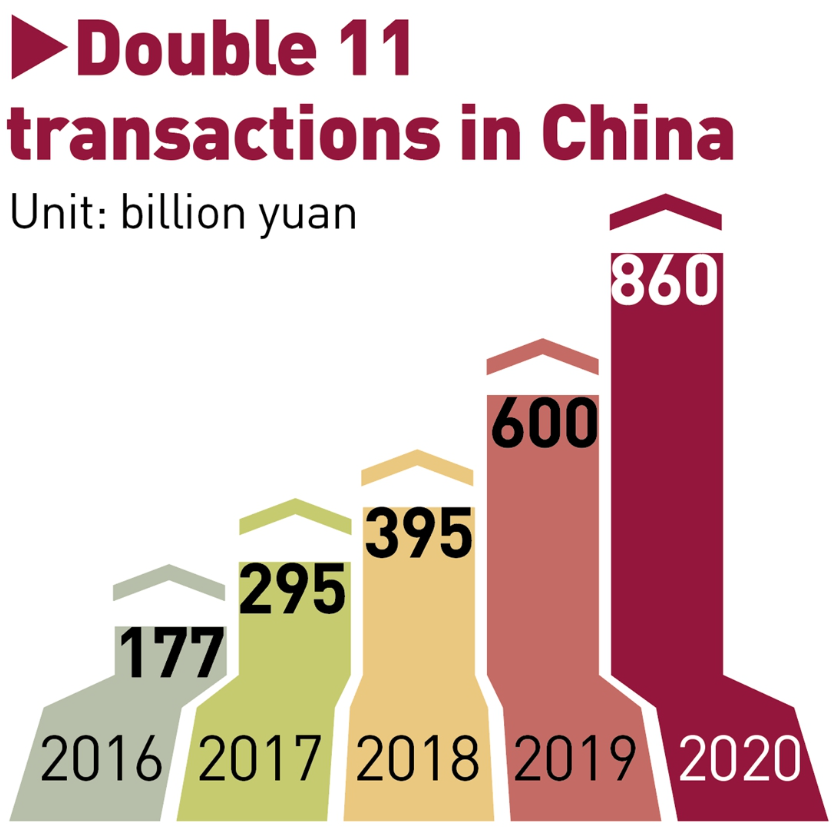
\includegraphics[width=\textwidth]{Images/1.png}
        \caption{2016-2020年“双十一”中国地区交易额\cite{1}}
        \label{double-ele}
    \end{minipage}
    \hfill
    \begin{minipage}[t]{0.65\textwidth}
        \centering
        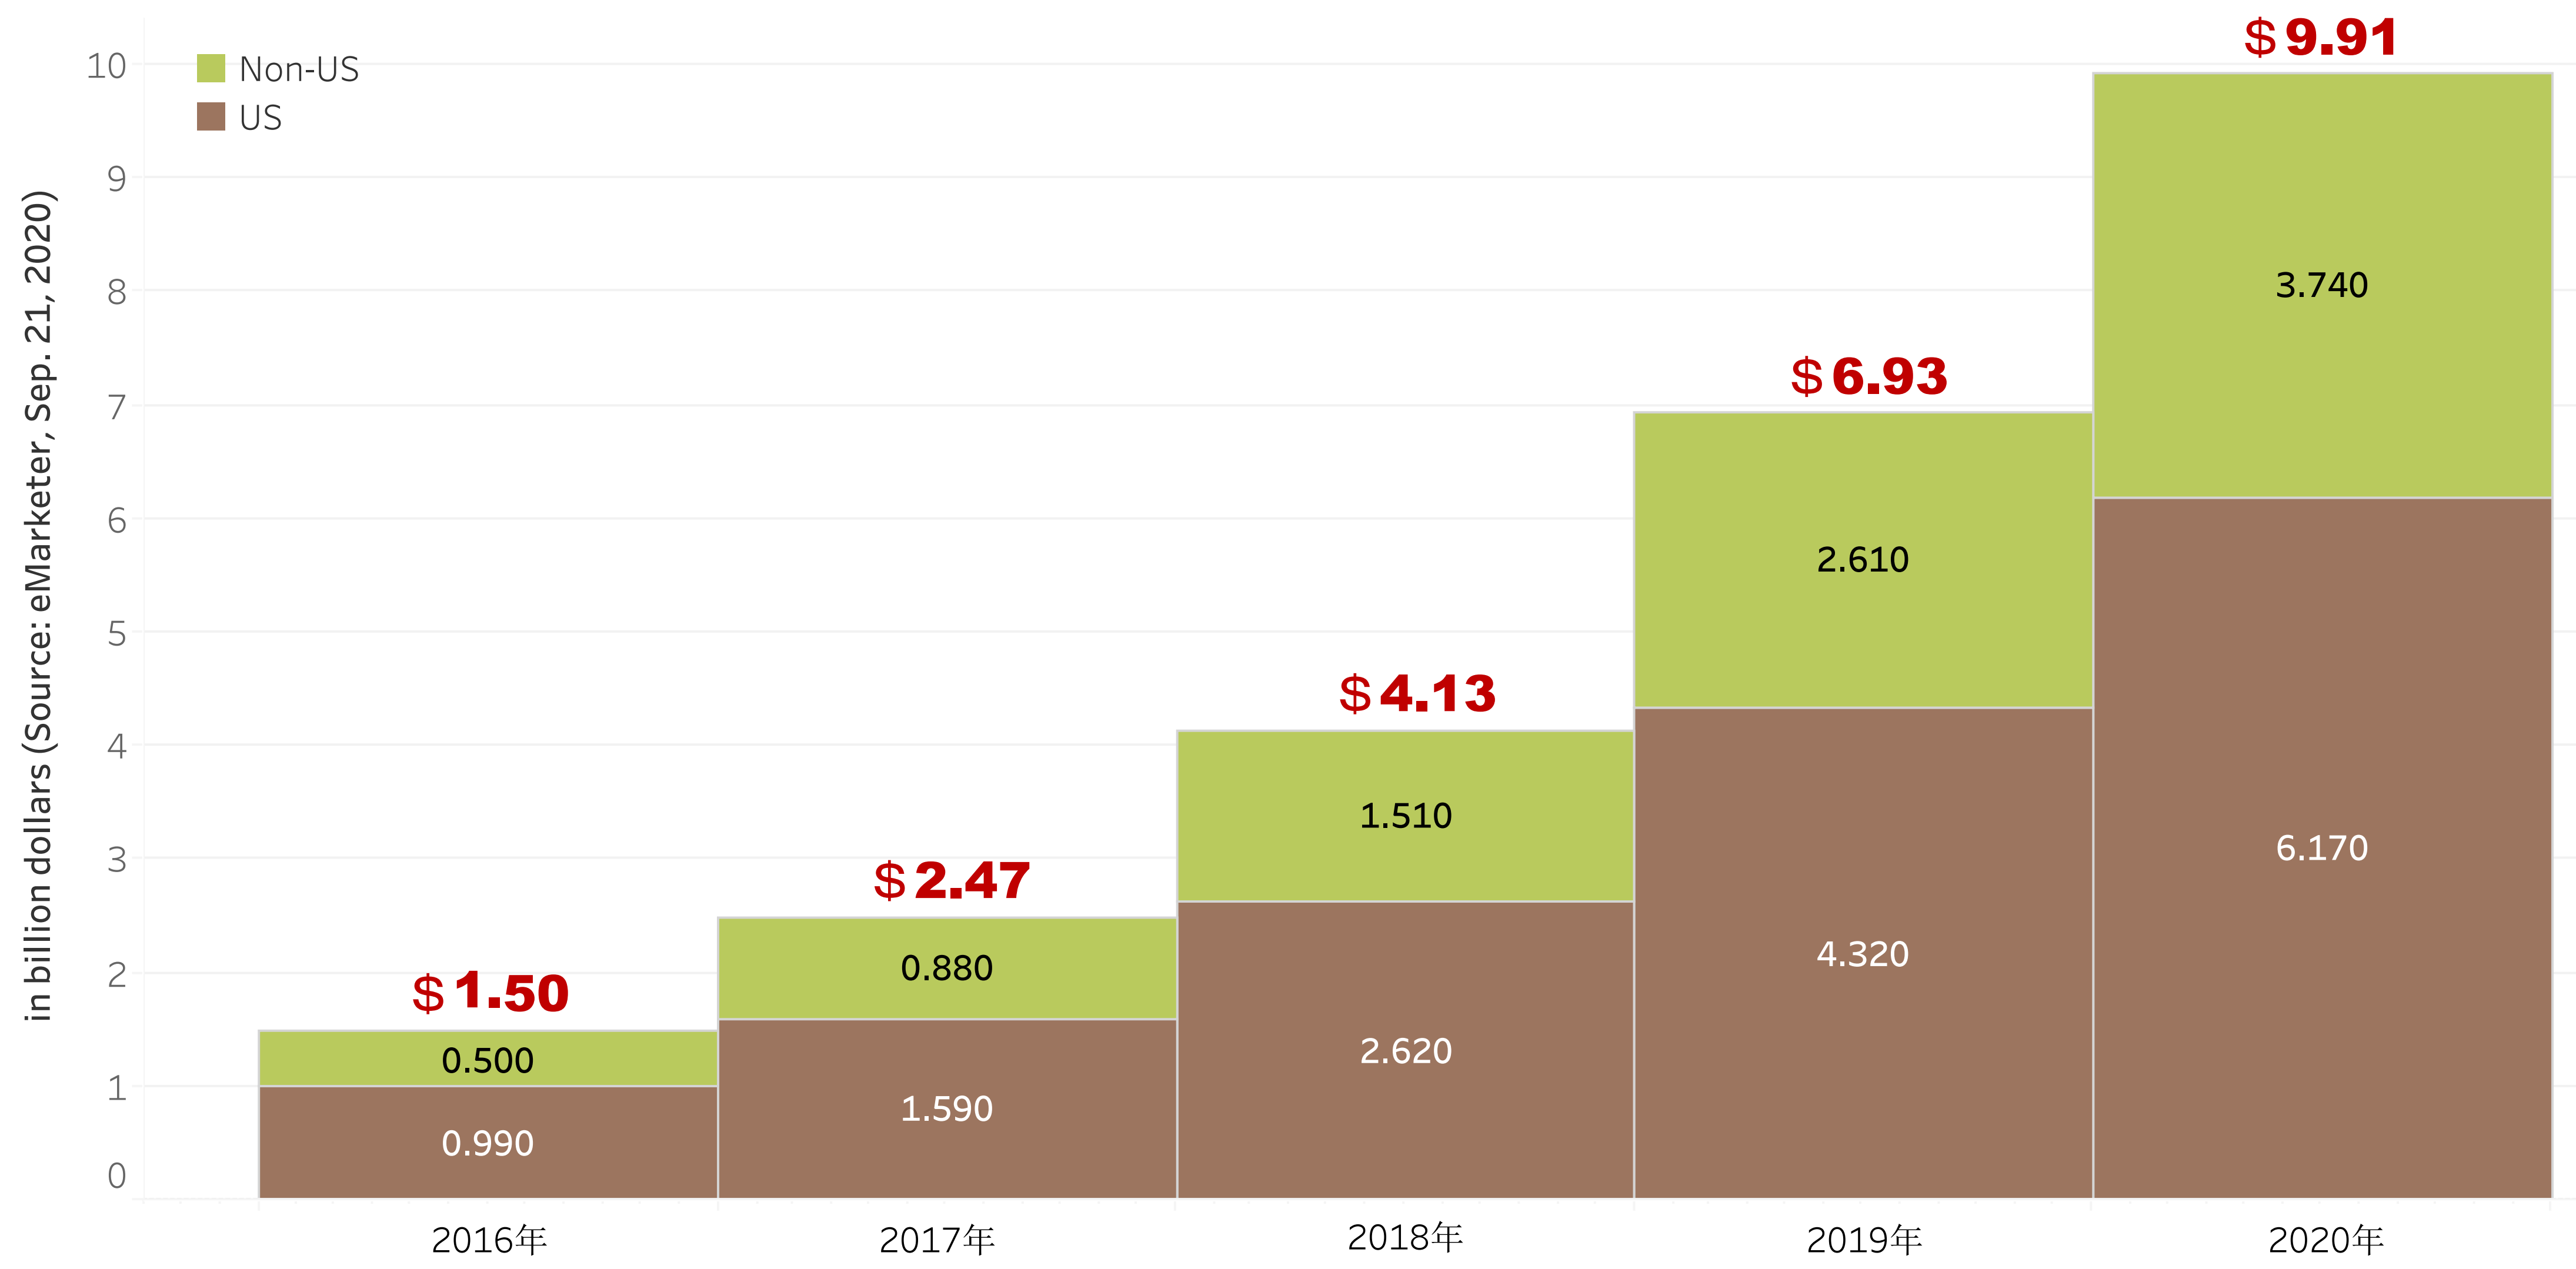
\includegraphics[width=\textwidth]{Images/2.png}
        \caption{2016-2020年Prime Day当天美国地区、非美国地区以及全球总销售额(数据来源:\cite{2})}
        \label{trd}
    \end{minipage}
\end{figure}

以“双十一”和Prime Day为例,在2020年前购物节当天的交易额都呈近指数式增长趋势。不难发现,许多购物节都依托于一些庆典类节日来设置,以此赋予它们实际意义,也就是Seth Godin所说的营销是关于“讲述的故事”。但这种魅力是永恒的吗?不见得其然。

购物节曾经是购物者的狂欢日,守着凌晨十二点的购物车、等着限时抢购的促销活动...,不过任何辉煌都不可能不迎来它的日落,近三年消费节似乎并不如以前一样吸引人了。

去年十一月的一篇消费者行为报告中就提到,通货膨胀成为了消费者行为变化的首要影响因素之一,生活成本愈加增高、购买力下降,这些从根本上改变了支出的动态,消费者则会在非必需品和必需品中选择后者,购物节的促销就稍显无力了。而且,越来越多的人开始节俭和有意识地消费,消费的重点不再仅仅在于积累,这实际上反映的是目的性更强、价值驱动的购买决策的转变。这一趋势标志着群众正在背离过度消费文化,并希望敦促企业将其产品与不断发展的良心消费主义精神相结合\cite{3}。以上提到的两个内、外驱动因素使得购物节的魅力大不如前。

\begin{figure}[htbp!]
    \centering
    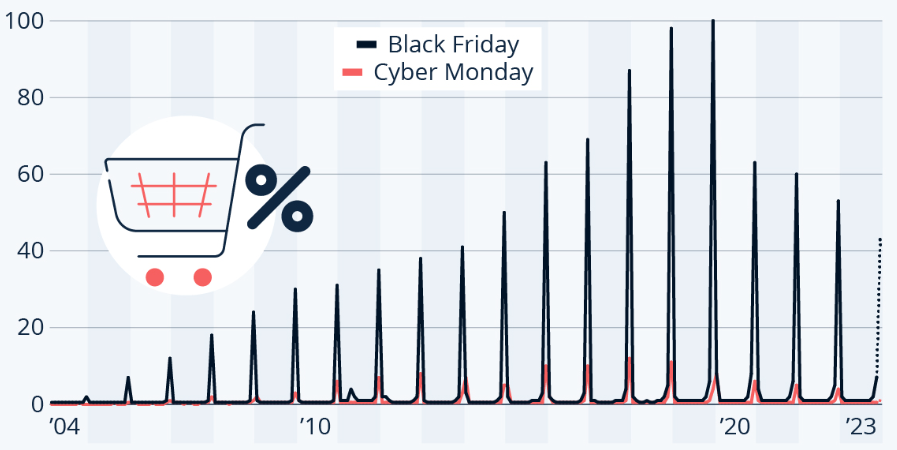
\includegraphics[width=0.9\textwidth]{Images/3.png}
    \caption{2004-2023全球谷歌搜索中“Black Friday”和“Cyber Monday”的搜索热度\cite{4}}
    \label{bf-cm}
\end{figure}

如图(\ref{bf-cm})所示,2020 年 11 月,谷歌中“Black Friday”一词的搜索热度比 2019 年下降了 30\% 以上,且这种下降趋势还将持续。在\cite{4}中,Statista的数据记者Felix Richter对这种趋势给出的理由是:优惠已无处不在,消费者不再需要等到购物节。

\subsubsection{案例分析:Black Friday}
TIDIO在今年9月发布的一篇调研报告\cite{5}中称,在2023年的Black Friday,一共有1.34亿人在网上购物并花费了380亿美元,且有48\%的受访者都在为当天的消费提前攒钱。在美国,有7620万消费者涌入线下商店,相比2022年增长了4.6\%,使之成为年度最受欢迎的购物节。

虽然从消费数据来看,购物节仍然促成了消费的猛增,但人们对它的态度似乎并不是很好。约 84\% 的 Z 世代购物者认为Black Friday的优惠很划算,但他们中的 60\% 会对购物感到后悔;而对婴儿潮一代,也有 40\% 的人对自己在节日期间的消费方式不认可。大多数消费者认为“Black Friday”只是一个骗局,其所带的消费主义色彩过于浓厚,目的是让人们花比平时更多的钱,还有23\% 的受访女性认为零售商在假期前会人为地提高价格,又在购物节当天再次降价。但矛盾的是,仍然有57\% 的受访者认为今年人们的购买力会增强,38\%的人还表示自己准备花更多的钱。

不妨以2020年为分界线,看看前后人们对Black Friday的看法的转变\footnote{左图使用的百分比计算公式为 $\bar{p}_i=\sum_{j=1}^{4}p_{ij}\frac{n_{\cdot j}}{N}$,为各个地区内占比的加权和,其中$n_{\cdot 1}=771$(美国)、$n_{\cdot 2}=393$(英国)、$n_{\cdot 3}=393$(德国)、$n_{\cdot 4}=409$(加拿大),保留至第三位小数。右图$N=598$比左图样本量少。}。

\begin{figure}[htbp!]
    \centering
    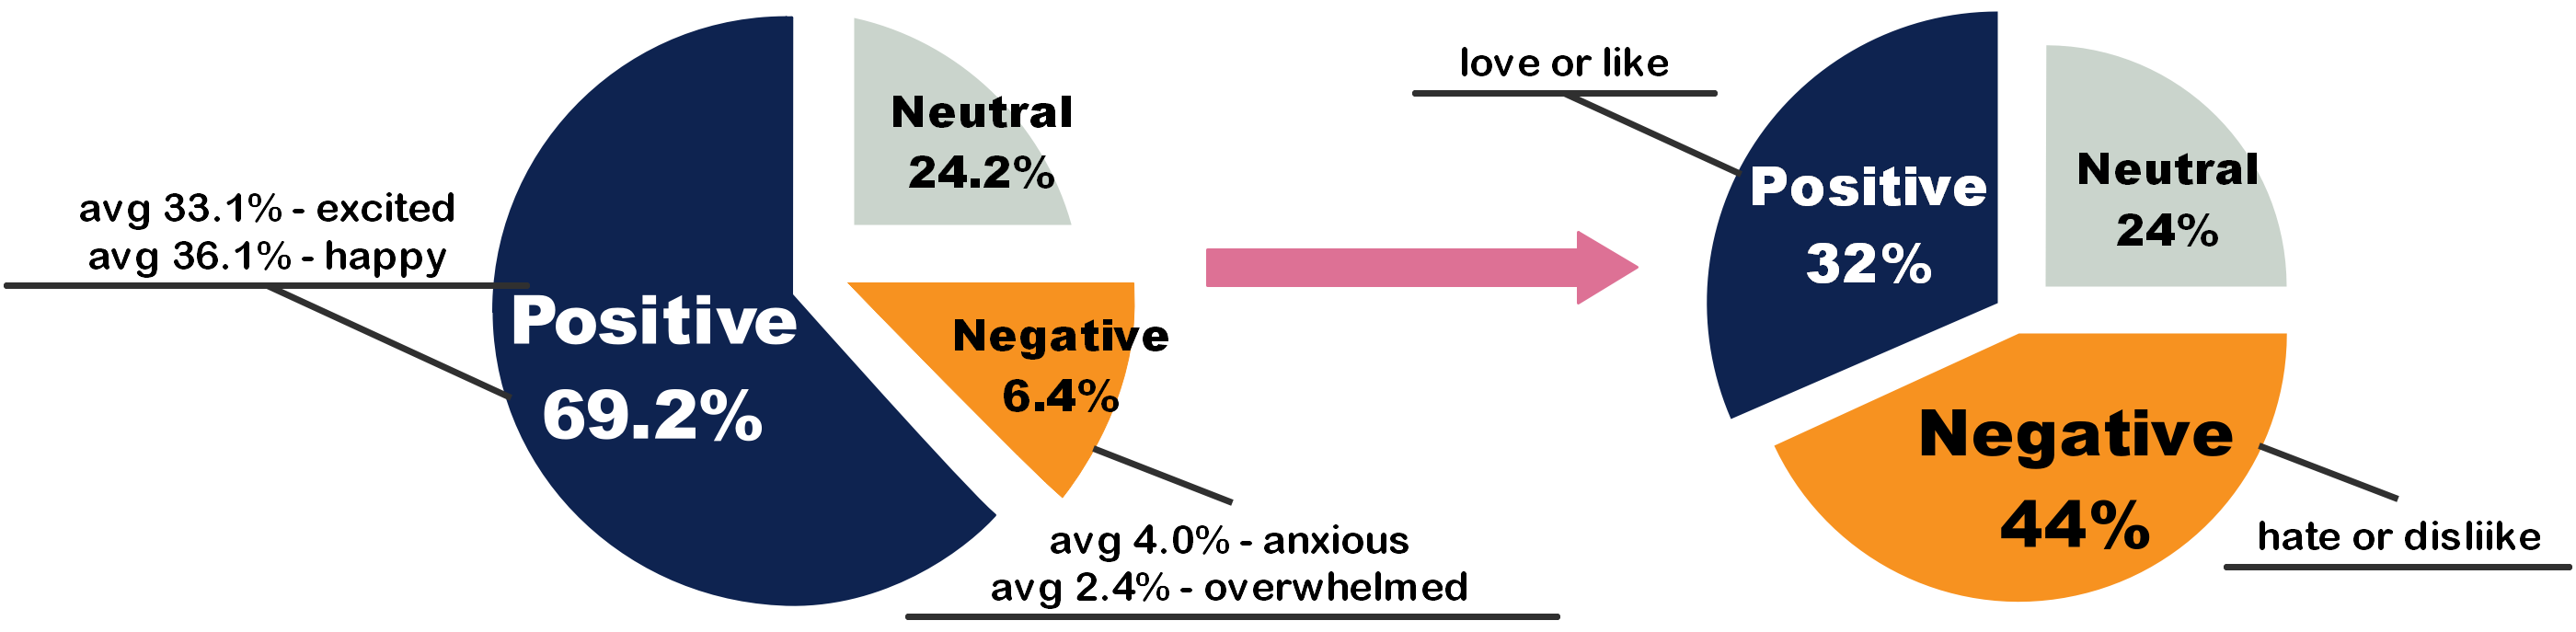
\includegraphics[width=1\textwidth]{Images/4.png}
    \caption{2018年9月(美国、英国、德国、加拿大地区)受McKinsey \& Company调研与近期受Survey Monkey调研的消费者对Black Friday购物节的感受(数据来源:\cite{6,7})}
    \label{pnn}
\end{figure}

由图(\ref{pnn})易见,持中立态度的人数占比几乎没有变动,但原本持正面态度的消费者则转向了持负面态度,且其占比甚至超过了持正面态度的人数占比(至接近50\%)。

在谈论到为什么不喜欢Black Friday的问题,\cite{6}的调研结果做了一个简单的归因。

\begin{figure}[htbp!]
    \centering
    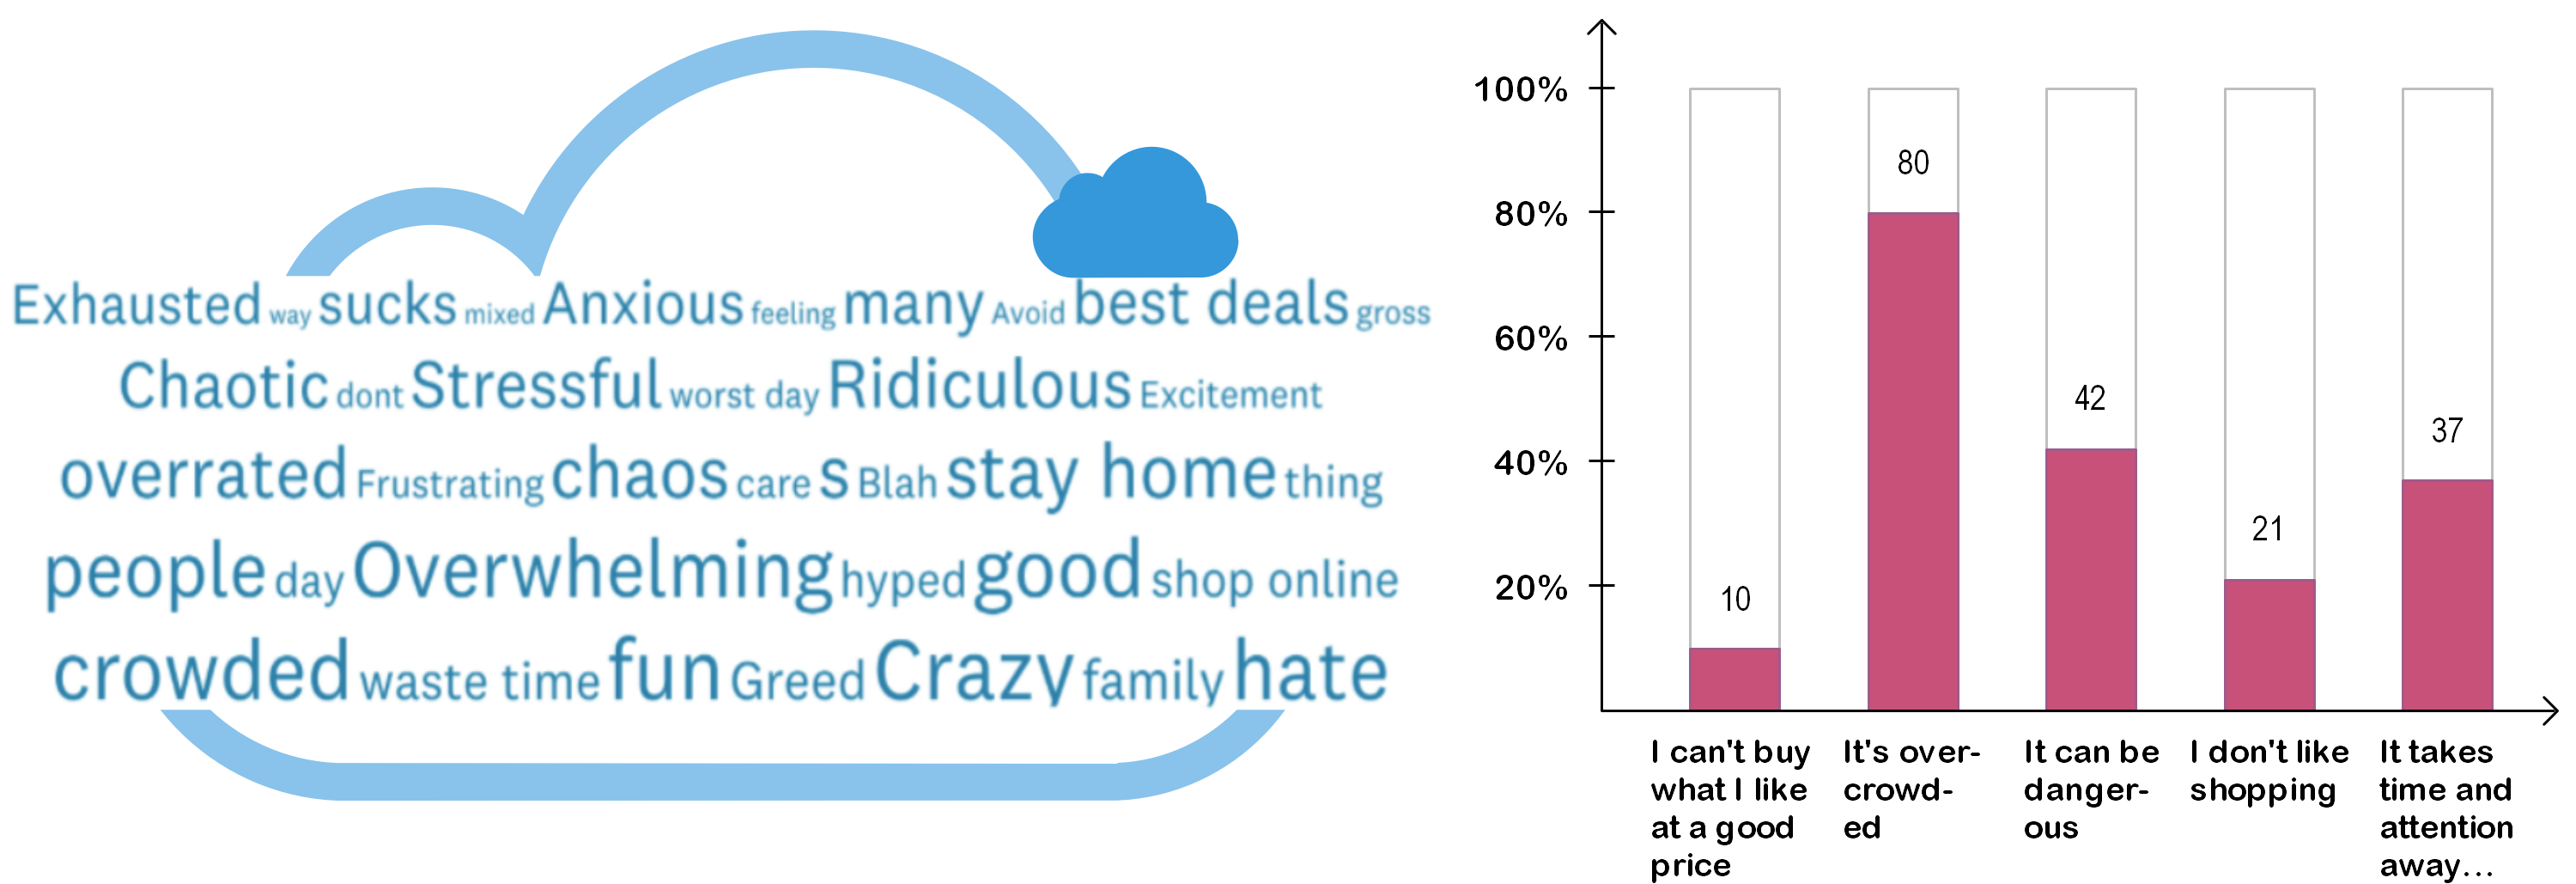
\includegraphics[width=0.95\textwidth]{Images/5.png}
    \caption{“哪个词最能概括你对Black Friday的感受?”自由回答问题词云与人们不喜欢Black Friday的理由(词云图、数据来源:\cite{6})}
\end{figure}

“Overwhelming”、“Crazy”、“crowded”、“Ridiculous”、“hate”、“Chaotic”...调研词云最突出的几个词都是负面评价,从右边的多选统计图表中还能看出,约五分之四的人是因为过于拥挤而不喜欢Black Friday,排名第二的原因是很危险(对应词云中的混乱、疯狂等),紧随其后的一点是其挤占了消费者大量的精力和时间,也就是说他们更愿意去做别的事而不是购物。

除此之外,虽然最不愿意花大钱在Black Friday的为60岁以上的人,年轻人接受度更好,但他们并不愿意将它与其他年度活动相提并论,83\% 的 18-29 岁年轻人都不认为这是一项传统\cite{6}。在缩减开支的近几年,年轻消费者希望广告是发自内心的,而不是大肆炫耀财富,他们还会监控交易,看看哪些有价值,哪些没有价值,并比较其他网站上的产品寻找最大折扣\cite{8}。

\subsubsection{案例分析:Cyber Monday}
Cyber Monday是Black Friday后的第一个星期一,是为了推动在线购物而设立的购物节,而Cyber Week则是Cyber Monday促销时间的延续。很明显,它的趋势与Black Friday十分相似,根据2021年CNBC的报道\cite{10}和图(\ref{cm})来源于Adobe Analytics的数据,当天的总消费额较去年同期下降 1.4\%,迎来历史上的首次下降。但是消费似乎是分散到了Cyber Week上而不再是集中在Cyber Monday当天,总销售额仍然呈上涨趋势。

\begin{figure}[htbp!]
    \centering
    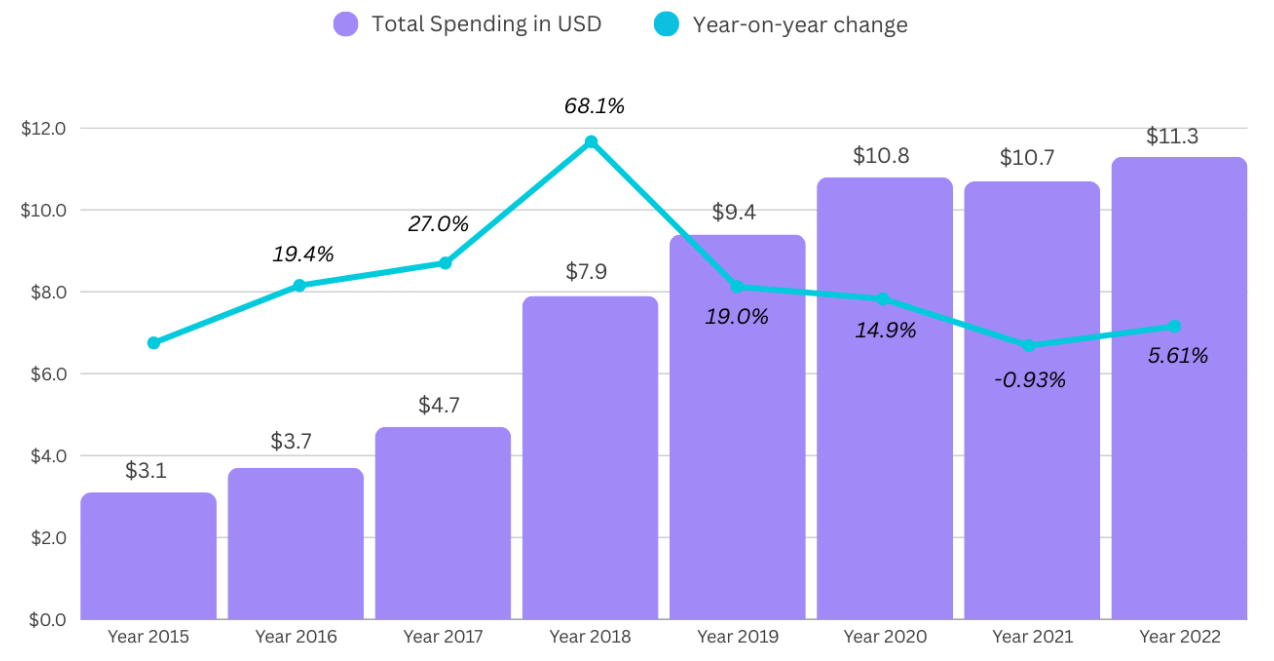
\includegraphics[width=0.9\textwidth]{Images/6.png}
    \caption{2015-2022年Cyber Monday总消费额(单位:十亿美元)\cite{9}}
    \label{cm}
\end{figure}

随后的2022年,当天的销售额这一数值又在再度回升,在2023年达到121亿美元。考虑到Cyber Monday主攻线上销售的特殊性,不妨再细分一下。

\begin{figure}[htbp!]
    \centering
    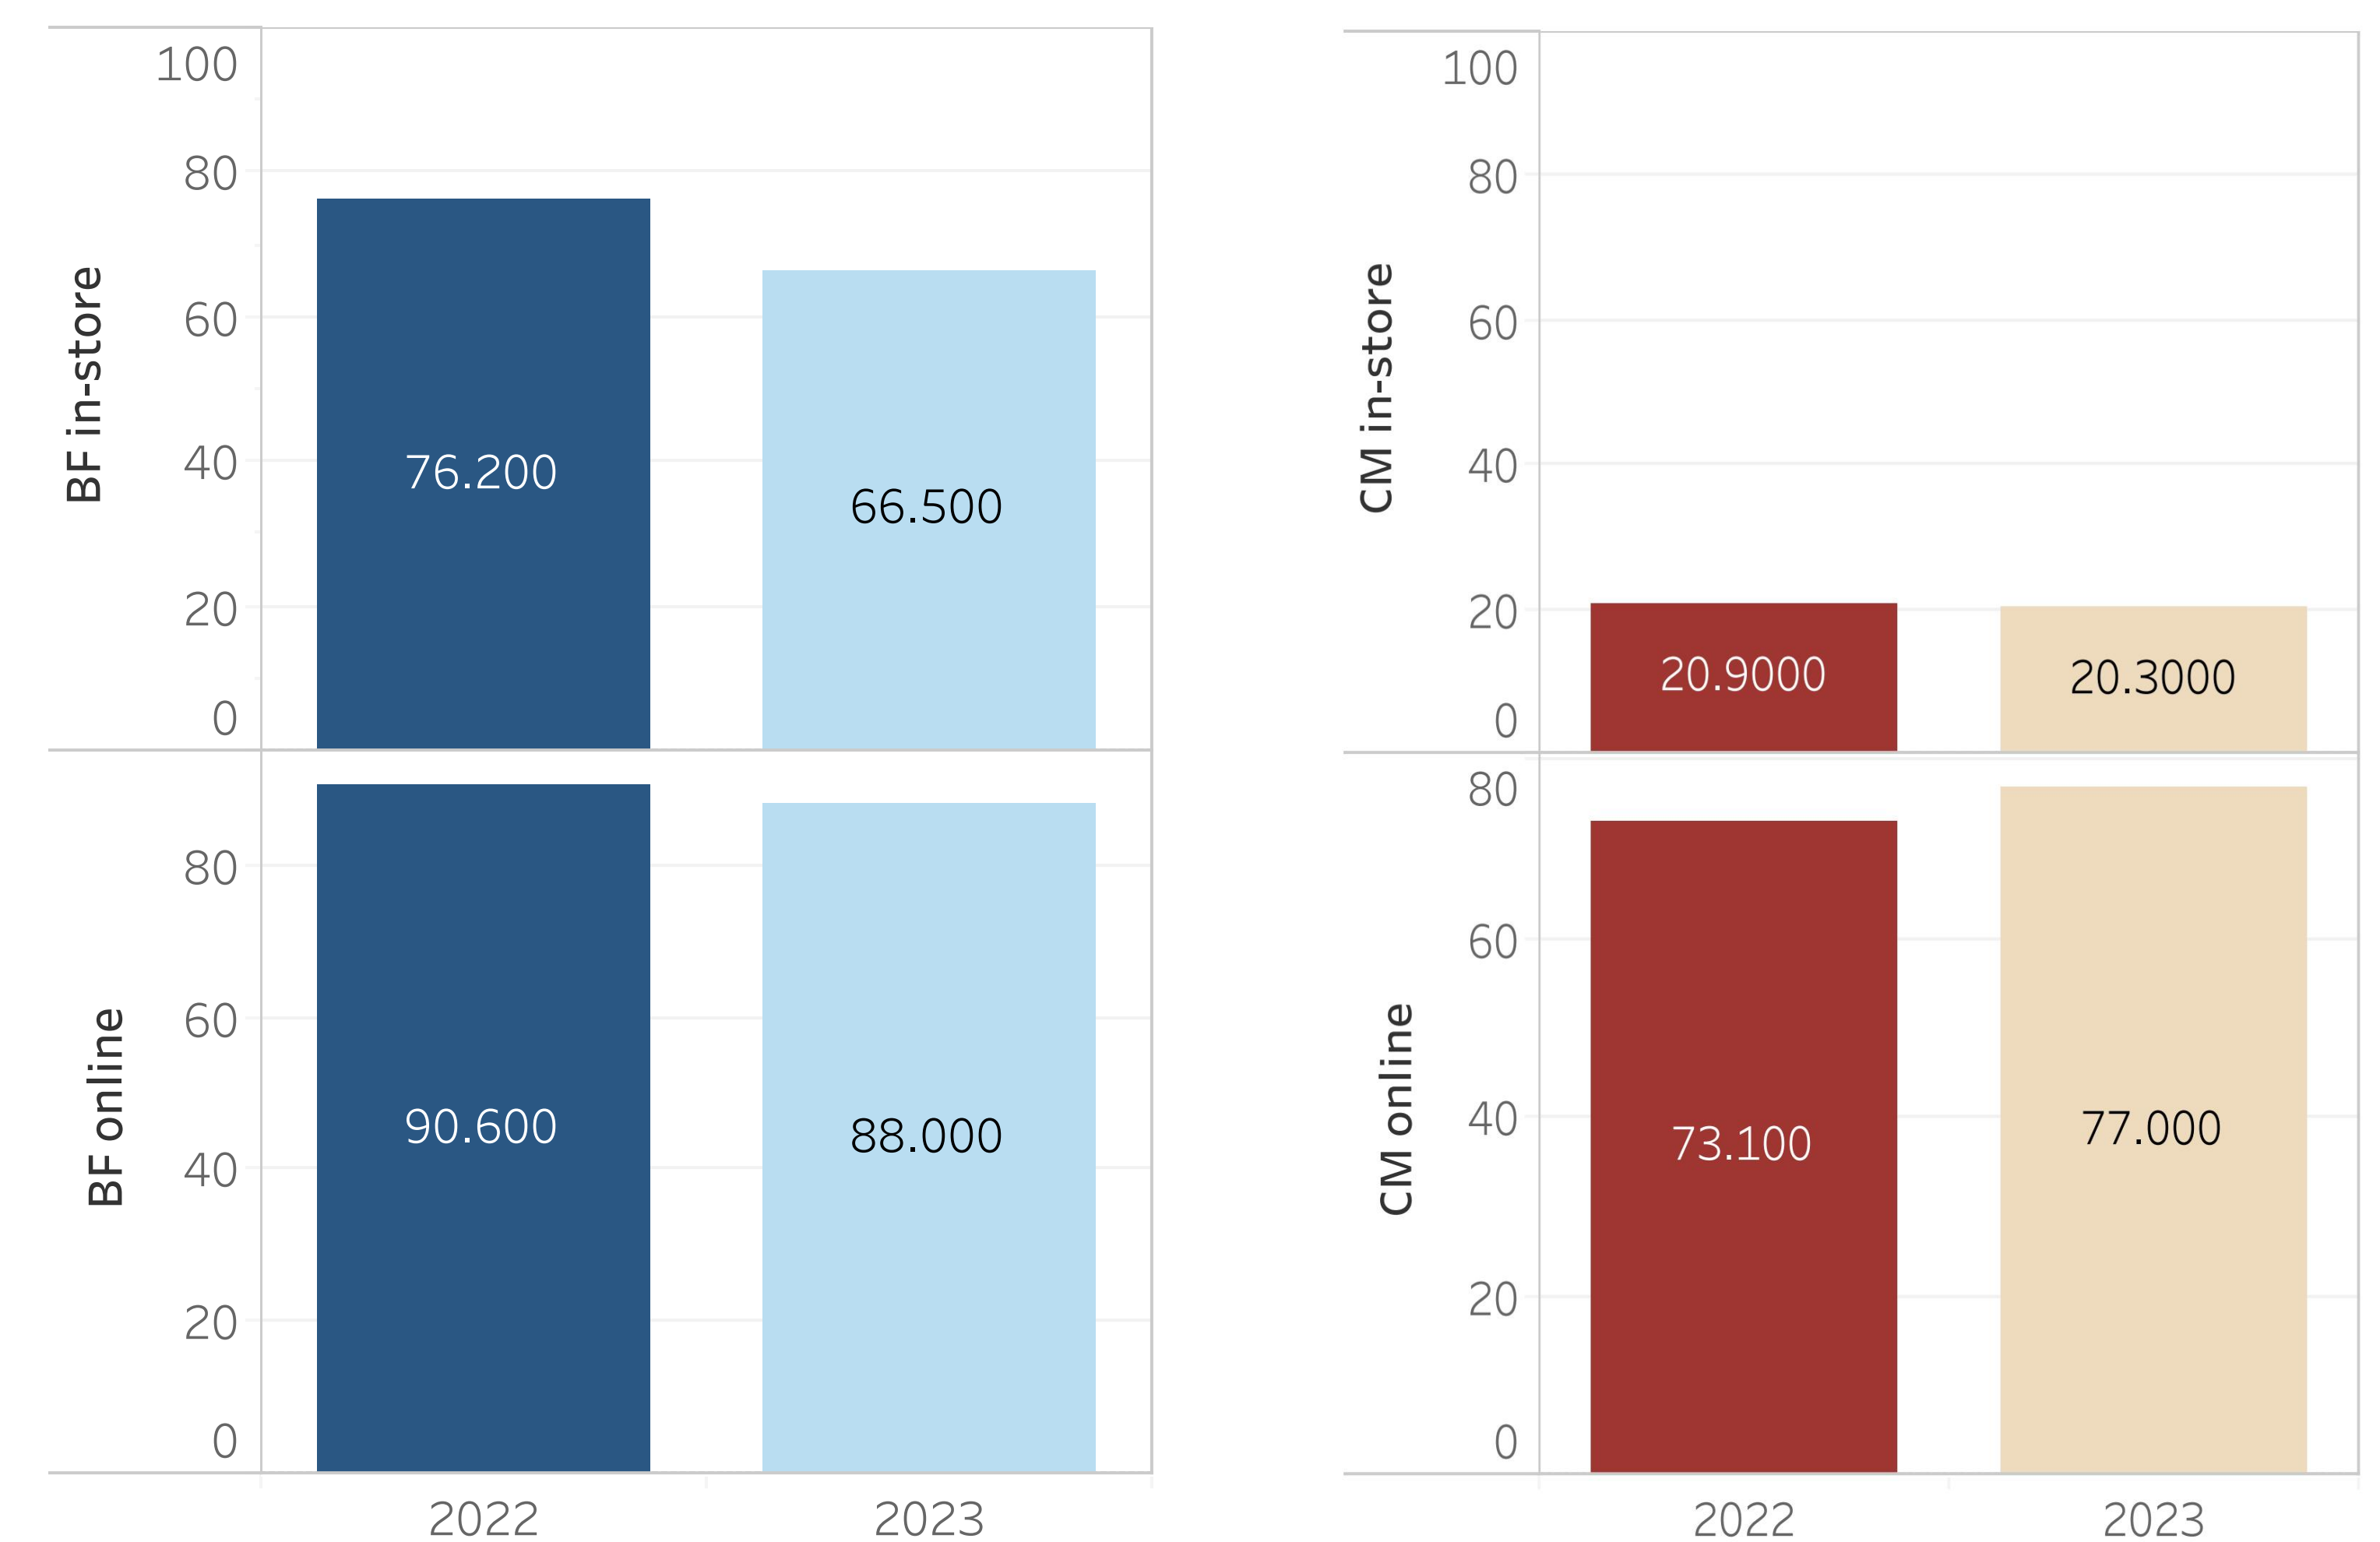
\includegraphics[width=0.8\textwidth]{Images/9.png}
    \caption{Black Friday、Cyber Monday线上线下销售额(单位:十亿美元)(数据来源:\cite{9,11})}
    \label{BFandCM}
\end{figure}

由图(\ref{BFandCM})的数据可以发现,Cyber Monday的线下购物销售额略有降低,但线上购物销售额却明显增长了,呈相反趋势。结合Black Friday的数据表现,可以推测相较传统线下购物节活动,更多人涌入了线上购物节,即使在购物节正在逐渐失去魅力的今天,这个由电商市场引领的进步也是无法忽视的。根据National Retail Federation2023年的报告,约有4050 万人使用手机进行网上购物,低于 2022 年创纪录的 4570 万人,但仍远高于疫情前的水平,不过人们对Cyber Monday的满意度值得存疑,NIQ的数据显示,有60\%的消费者都认为2023年的Cyber Monday优惠力度不如2022年,的确,许多商品的折扣力度不如之前。Forbes预测,今年的购物车放弃率将大幅上升,消费者愿意花更多时间研究和寻找优惠\cite{11},特定购物节将不再享有很高的关注度。

对Cyber Week购物活动而言,只有22\%的消费者计划增加比往年更高的假期购物预算\cite{12},这一归因之本仍然是过高的生活成和生活必需品的价格。

\begin{figure}[htbp!]
    \centering
    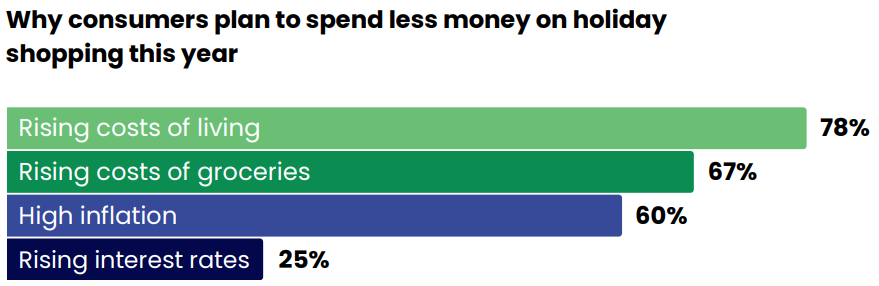
\includegraphics[width=0.75\textwidth]{Images/11.png}
\end{figure}

Techopedia认为,网络诈骗层出不穷也是影响消费者对购物节(尤其是线上购物节)的满意度、从而间接导致购物节消费增长的停滞的一大原因。

\begin{figure}[htbp!]
    \centering
    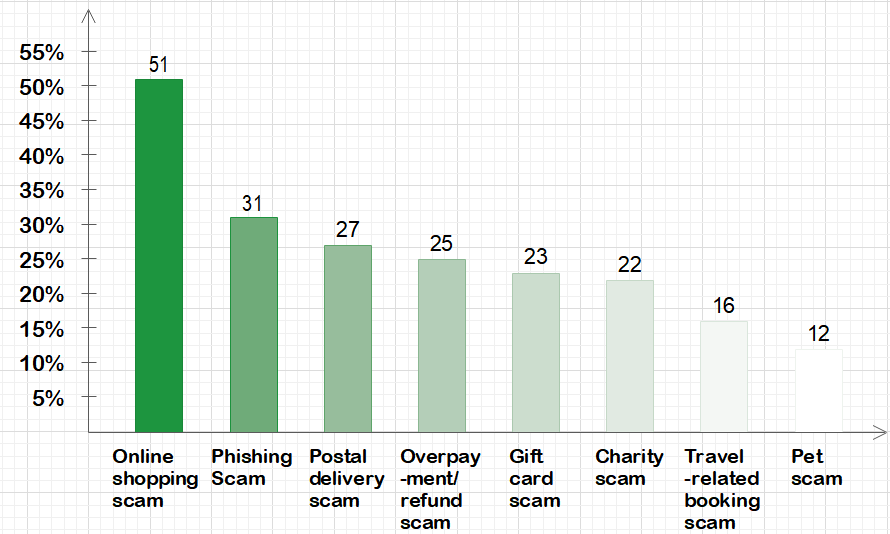
\includegraphics[width=0.7\textwidth]{Images/10.png}
    \caption{2023年所经历的网络诈骗(数据来源:Norton 2023, \cite{11})}
    \label{scam}
\end{figure}



\subsubsection{案例分析:Prime Day}
Prime Day虽为后推出的购物节活动,但因其依托于亚马逊Prime服务,因此十分受青睐。

由eMarketer预测的数据可以看出,2021年起,Prime Day的销售额增长率突然陷入了低迷状态,预计到今年将降低至6.4\%,这一增幅成为了近三年的最低,也远不及2020年的43\% \cite{12}。

\begin{figure}[htbp!]
    \centering
    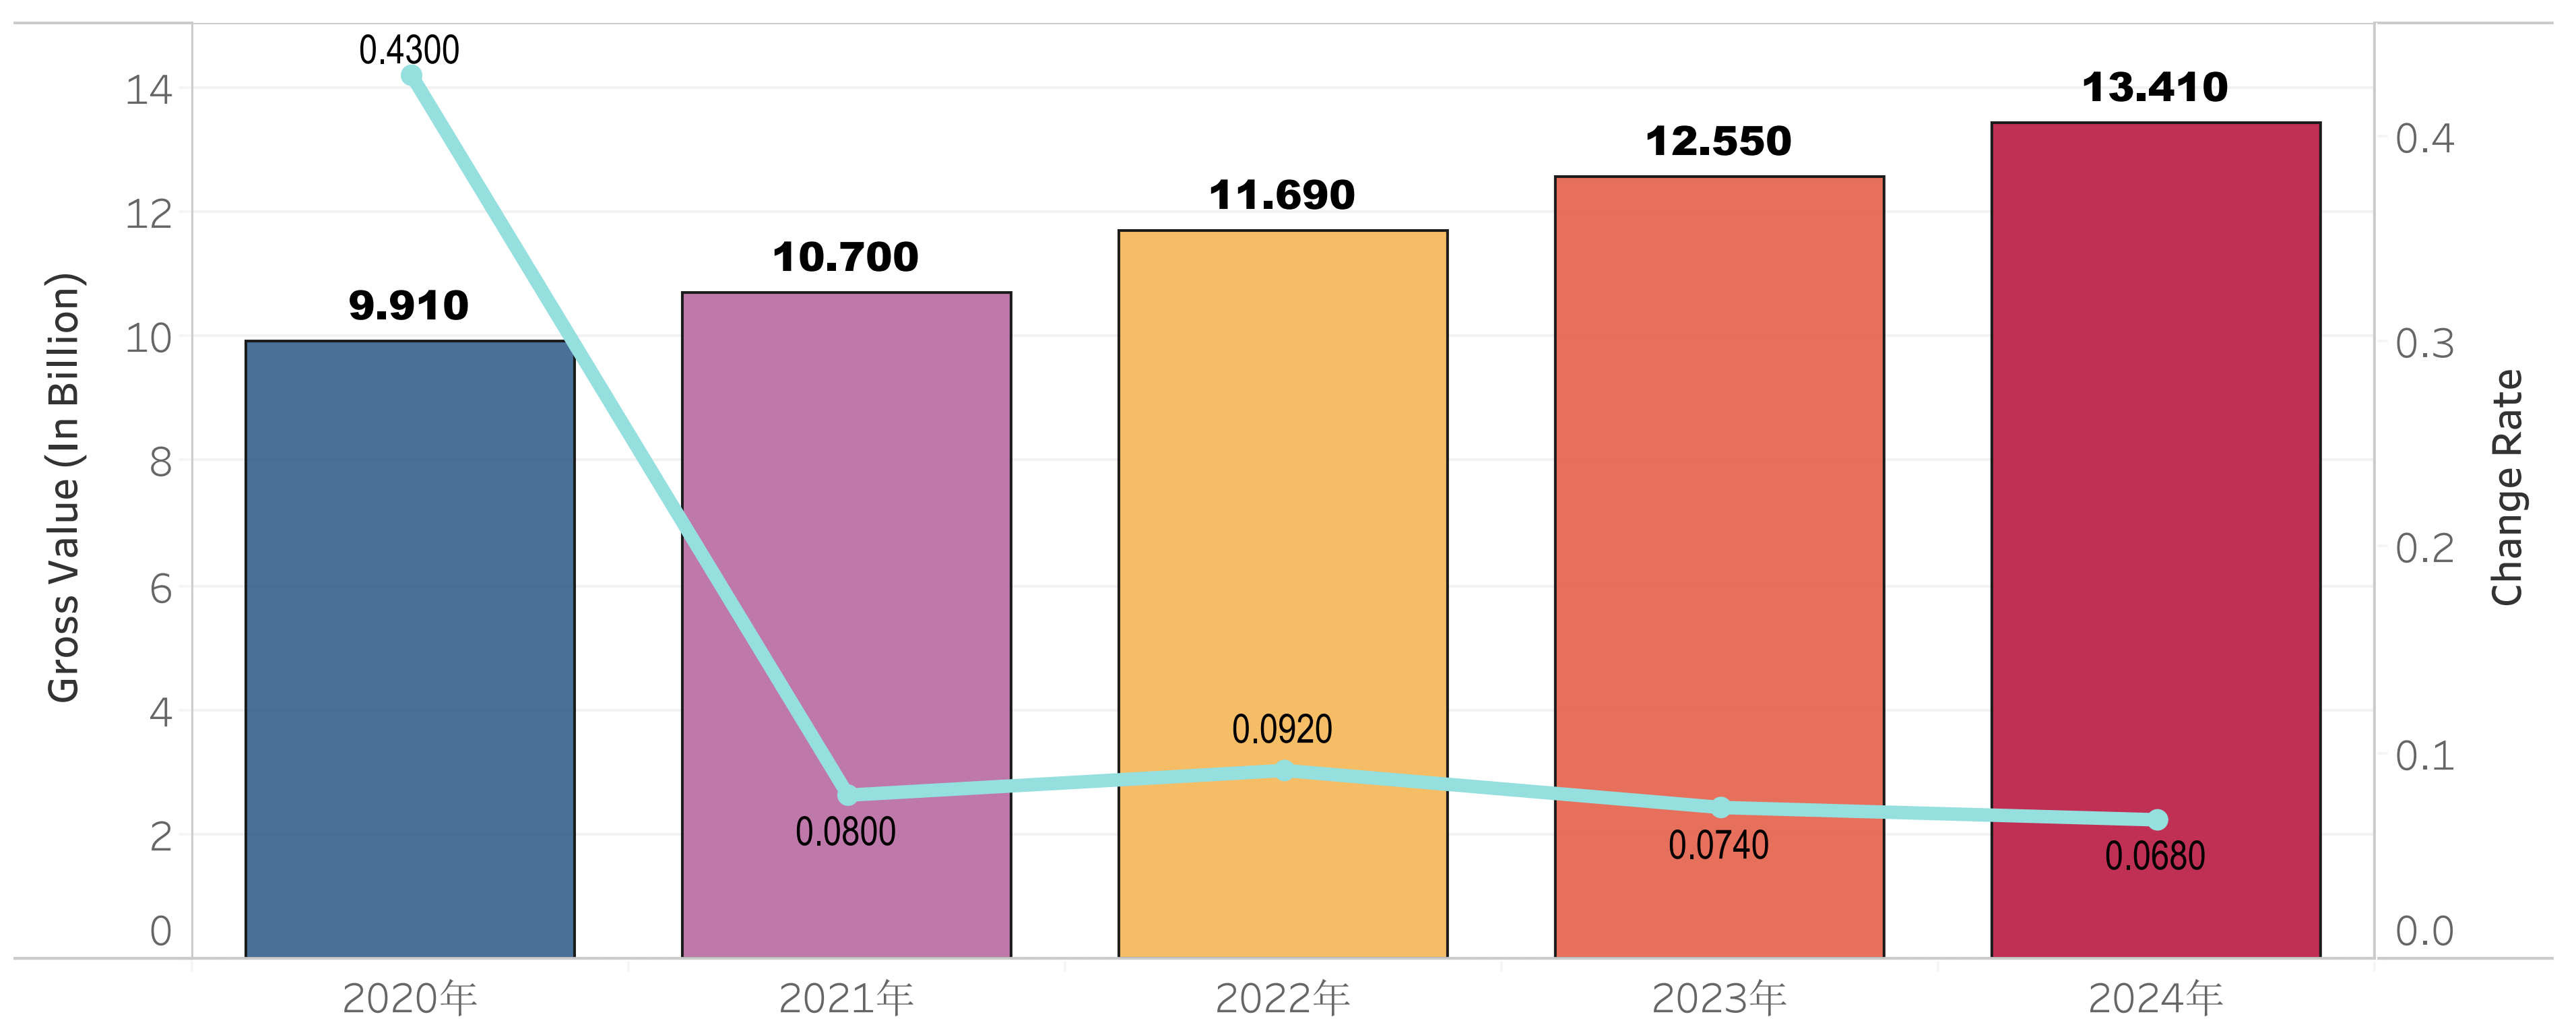
\includegraphics[width=0.8\textwidth]{Images/12.png}
    \caption{2020-2024年全球亚马逊Prime Day当天的销售情况(数据来源:\cite{12})}
    \label{scam}
\end{figure}

根据NIQ的2023年Prime Day调研结果,许多美洲、欧洲地区消费者也将Prime Day作为视为一种“存钱方式”,以使他们能够在通货膨胀带来的高价下暂时松一口气\cite{14}。

\begin{figure}[htbp!]
    \centering
    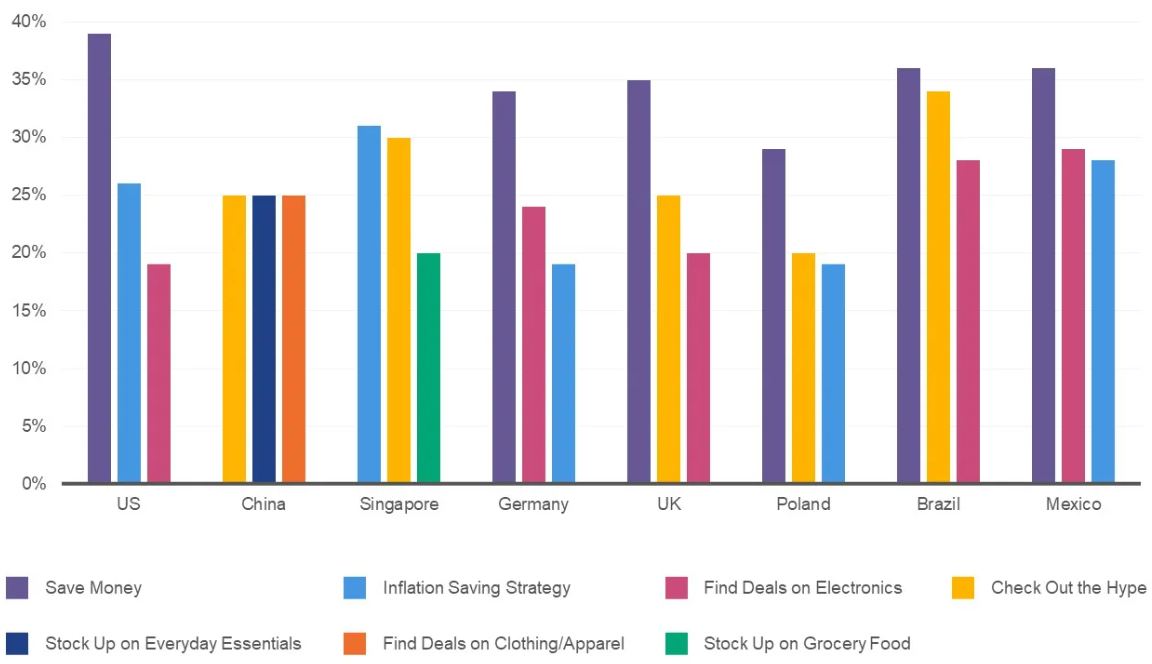
\includegraphics[width=0.8\textwidth]{Images/13.png}
    \caption{2023年Prime Day各主流地区不同动机购买的受访者占比 \cite{14}}
    \label{purpose}
\end{figure}

图(\ref{purpose})中,似乎只有中国地区消费者还仍然仅将Prime Day作为购入日需品、服装、了解当前热议的途径,其他地区都有超过三分之一的消费者以此达到“存钱”或应对通货膨胀的目的。购物节已经不再仅仅是人们购物狂欢、大肆消费的节日了。

针对今年的Prime Day,eMarketer给出了如下几个消费者对于购物节的情绪变动\cite{15}:
\begin{itemize}
    \item \textbf{目的明确与实用性盖过购买行为.} \\
    根据 CivicScience 2024 年 7 月的数据,今年近四分之三 (74\%) 的 Prime Day 购物者购买了个人或家庭必需品(如垃圾袋等),高于去年的 60\%;其他类型产品则显得寡淡无味。
    \item \textbf{需求预测与提前规划.} \\
    根据 Skai 2024 年 5 月的数据,超过六成消费者(62\%)在 Prime Day 之前研究过优惠活动,也就是说他们提前做过计划,在当天冲动消费的可能性更小;且随着亚马逊各个竞争对手的崛起,越来越多的消费者“愿意等待”,对购物节不再有紧迫感,而采用更明智的消费态度。
    \item \textbf{犹豫不决的温和决策.} \\
    购买返校用品、节日用品或礼物的消费者行为更加温和了。根据 JLL 2024 年 6 月的一份报告,超过一半(55.3\%)的美国父母计划减少返校用品支出,其中的三分之一将此决定归因为通货膨胀的适应性策略。
\end{itemize}


\subsubsection{案例分析:“双十一”}
“双十一”购物节由阿里巴巴旗下的淘宝推出,逐渐发展成为了中国乃至全球的购物盛会。

近三年,“双十一”当日成交额稳步上升,Deloitte数据显示,天猫双十一累计成交额5403亿元,同比增长8.45\%;京东双十一累计下单额3491亿元,同比增长29\%,抖音、快手等直播电商平台累计成交额2151亿元,较去年的1814亿元同比增长146.1\% \cite{16}。但它也同样难逃全球经济波动影响,如图(\ref{double})所示,从2021年起,全网成交额增长率突然下跌,至2023年已低至2.10\%。

\begin{figure}[htbp!]
    \begin{minipage}[t]{0.5\textwidth}
        \centering
        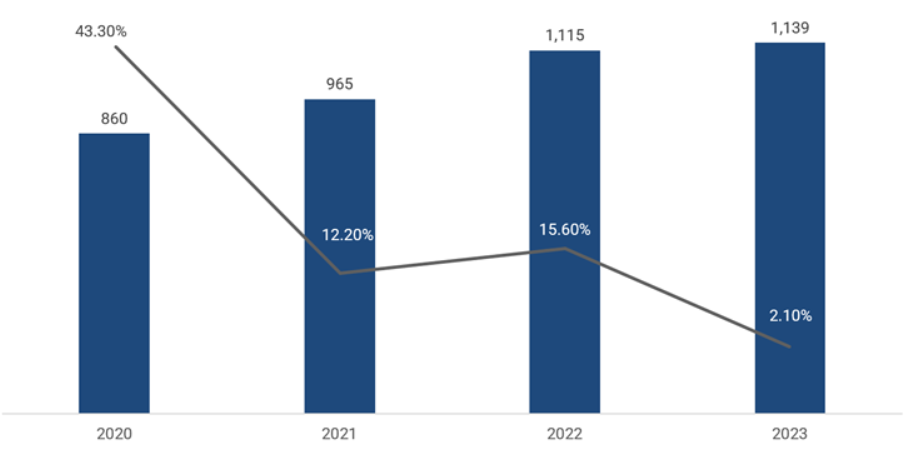
\includegraphics[width=\textwidth]{Images/14.png}
        \caption{2020-2023年“双十一”期间全网成交额及增长率(单位:亿人民币)\cite{16}}
        \label{double}
    \end{minipage}
    \hfill
    \begin{minipage}[t]{0.45\textwidth}
        \centering
        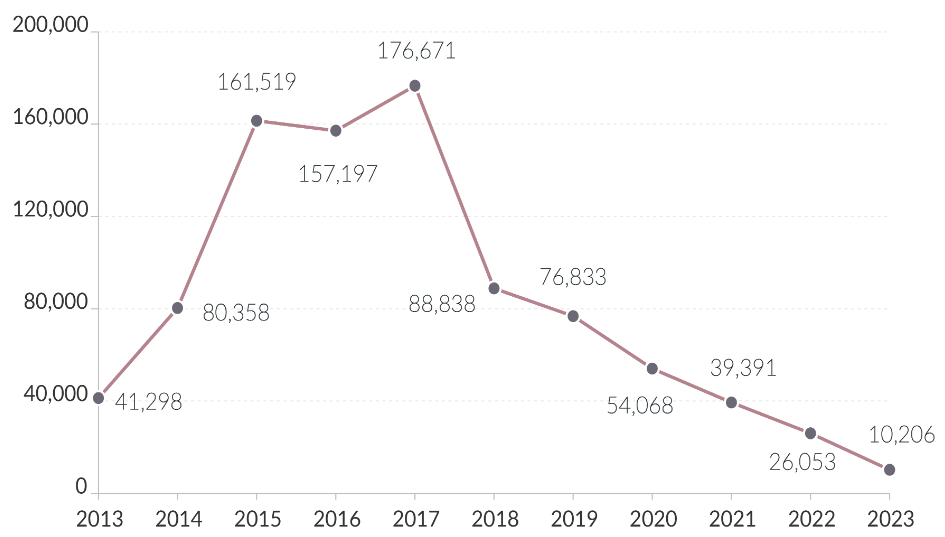
\includegraphics[width=\textwidth]{Images/15.png}
        \caption{2013-2023年百度引擎“双十一”词条搜索热度变化 \cite{17}}
        \label{cite}
    \end{minipage}
\end{figure}

“双十一”是否还如往常那样令消费者们着迷呢?可以猜测结论是否定的,如图(\ref{cite})的数据,从2018年开始,“双十一”的百度搜索热度就下明显下降了,直到2023年它的热度甚至不及十年前的四分之一。早在2021年,就有人根据Six Tone发布的数据发现,“双十一”经济放缓了,越来越多的人表达了他们对多年来积累的折扣却得不到任何好处的不满,“我们都厌倦了平台的游戏”一位Six Tone的分析师说。这还促使了反消费主义群体的诞生,曾有一个名为“不要买”的网络群组在一年内就拥有 30 万名成员,分享理性购物策略等 \cite{18}。


\begin{figure}[htbp!]
    \begin{minipage}[t]{0.45\textwidth}
        \centering
        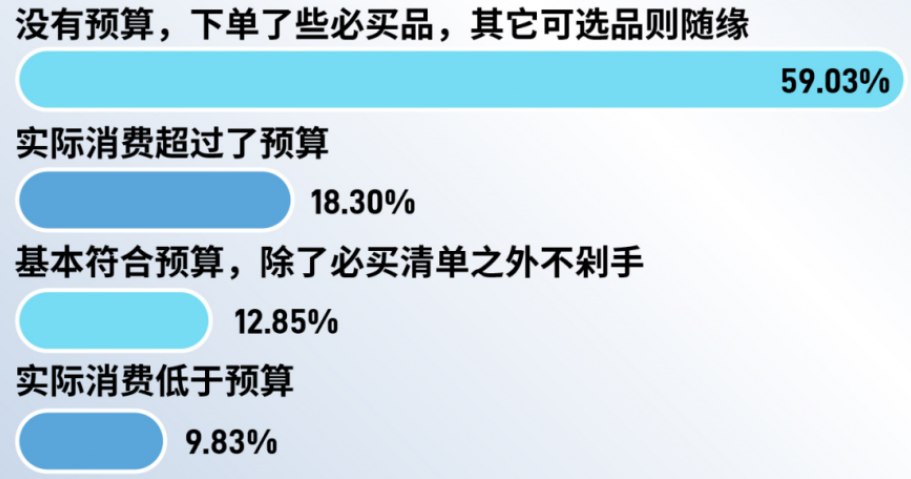
\includegraphics[width=\textwidth]{Images/16.png}
        \caption{“今年双十一,您的消费与计划预算相比(单选)”回答分布\cite{19}}
        \label{budget}
    \end{minipage}
    \hfill
    \begin{minipage}[t]{0.43\textwidth}
        \centering
        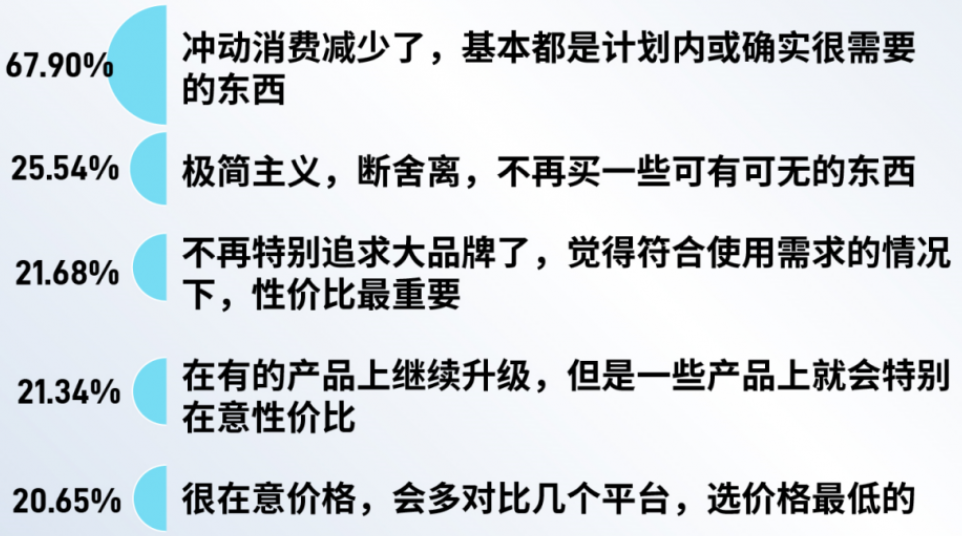
\includegraphics[width=\textwidth]{Images/17.png}
        \caption{“下列哪项符合您今年的消费决策?(多选)”回答分布 \cite{19}}
        \label{decide}
    \end{minipage}
\end{figure}

根据2023年21世纪经济报道“双十一”购物节的调研结果($N=1300$),“健康”和“文化”两个关键词是新的消费趋势。图(\ref{budget})和图(\ref{decide})都表明大部分消费者不再追求购物行为,且奉行极简主义生活。类似的,Deloitte的2023年白皮书\cite{20}的调研结果揭示了消费者对购物节的态度变化:(1) 理性、务实 - “真实需要”、“性价比”、“对人类社会负责任”是消费观念排名前三;(2) 绿色可持续 - 环保低碳生活方式得到支持,甚至不乏消费者愿意为绿色消费而支付溢价。

针对“双十一”还有比较特别的一点,Bain \& Company发布的报告\cite{21}中,直播或短视频等以内容为主导的电商平台异军突起,2021至2022年的“双十一”当天商品成交额增幅达到了146\%,但这似乎并不是消费者对购物节的兴趣增加的表现,淡漠消费节、分散消费仍是主流趋势。


\subsection{消费者态度的变化趋势}

前文已经大致提到了消费者的悲观态度,不妨横向看看消费者历年对购物节的态度变化。

\begin{figure}[htbp!]
    \begin{minipage}[t]{0.53\textwidth}
        \centering
        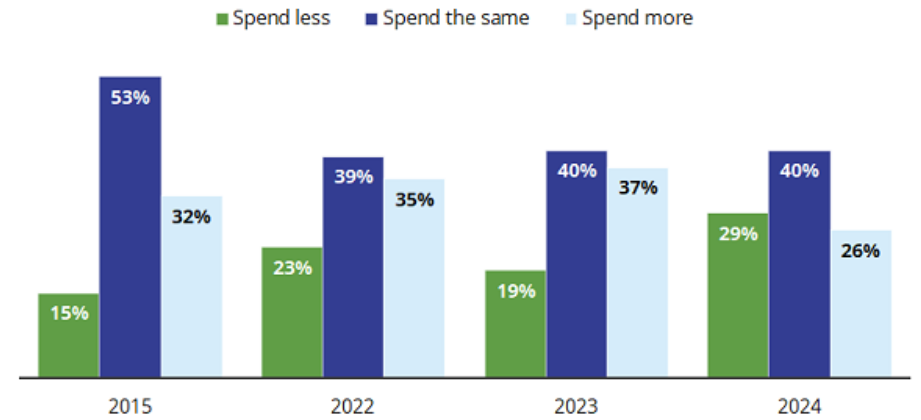
\includegraphics[width=\textwidth]{Images/20.png}
        \caption{2015、2022-2024 PwC的消费者购物节意愿调研数据结果分布图 \cite{37}}
        \label{attitude_1}
    \end{minipage}
    \hfill
    \begin{minipage}[t]{0.43\textwidth}
        \centering
        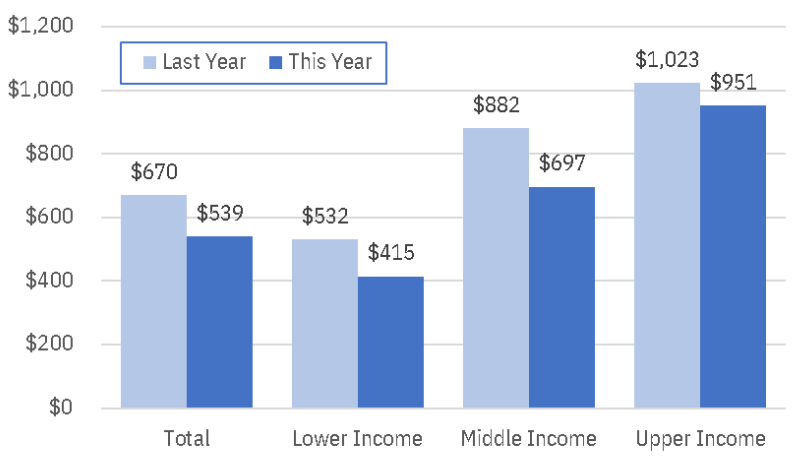
\includegraphics[width=\textwidth]{Images/21.png}
        \caption{2019-2020 IBM的消费者购物节意愿调研数据结果 \cite{38}}
        \label{attitude_2}
    \end{minipage}
\end{figure}

图(\ref{attitude_1})和图(\ref{attitude_2})显示的结果都是相同的,前者说明愿意花费与去年等同或更多的钱参与购物节的人数占比呈“减-增-减”的趋势,但总体仍然是下降状态,尤其是愿意花费更多的钱的消费者占比在2023年一度跌落至26\%;后者则是从平均预估花费的角度出发,更加直接地阐述了这一趋势,且不论家庭收入水平,都是较去年下降的,只是中低收入家庭预估开支削减地更明显。

但是有个奇怪的现象,人们似乎并没有很排斥“去参与”购物节,只是计划花的钱更少。

如图(\ref{attitude_3})所示,这是来自Boston Consulting Group的调研结果,各个地区“一定会参与”或“可能会参与”的人数占比其实是较2022年基本都有小幅度提升的,只有英国地区没有波动。澳大利亚和瑞士地区的“不参加”比例较其他地区更高,达到14\%;美国和波兰地区的“一定参与”比例也较其他地区更高,分别达到了40\%和39\%。


\begin{figure}[htbp!]
    \centering
    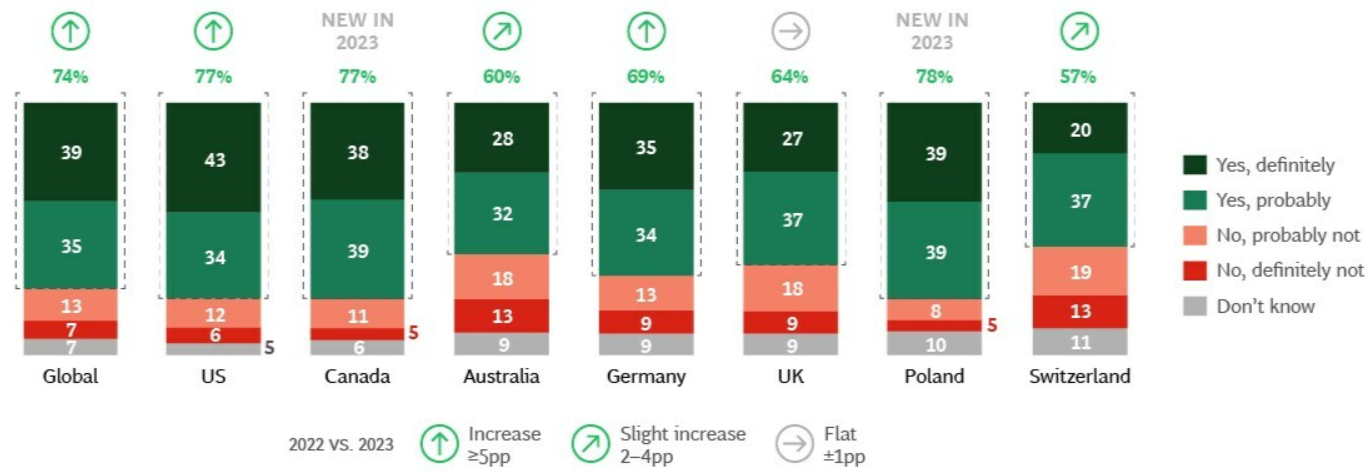
\includegraphics[width=0.9\textwidth]{Images/22.png}
    \caption{2022与2023年BCG的消费者购物节意愿(原问题:“Will you be shopping through the Black Friday/Cyber Monday/Single's Day shopping events being held in late Nov., 2023?”) \cite{39}}
    \label{attitude_3}
\end{figure}








\subsection{侦测消费者态度变化的内外因素}

前文在对几个经典的购物节的案例分析中都有对消费者态度变化的简单归因,现在不妨专门从成因层面分别探寻:到底是什么因素导致消费者不再热衷于购物节呢?

\subsubsection{外部 - 经济环境因素}
一个在前文反复出现的词语是“通货膨胀”。这是一个现实的问题,2023年6月的一篇报告\cite{36}中提到,通货膨胀上升,但工资却很少随之上涨,30\% 的消费者的未偿还债务比年初有所增加,50\% 的家庭要么勉强维持生计,要么无力维持生计,这一比例高于 2021 年 8 月的 40\%。消费者越来越意识到,随着社会生活必需品价格不断上涨,每月的预算会愈发紧张,因此他们必须决定如何最好地“节流”以降低最紧要的生活成本\cite{35}。

除了通货膨胀的问题,各大企业延长购物节、分散折扣的做法也反之使消费者不再关注购物节了。还记得每次品牌宣称这是购物打折的“最后机会”时,事实总是很少如此。2023年底Modern Retail的记者就提出了—“Black Friday”和“Cyber Monday”已失去意义——这一说法;RetailMeNot 的购物专家克Kristin McGrath认为,“零售商希望尽可能延长早期假日购物季,说服购物者多次前往,并在 12 月 25 日之后将货架上不想要的商品售罄。由于黑色星期五和网络星期一等促销活动充斥着大量宣传和紧迫感,零售商显然在试验他们能在多大程度上突破这些日子的界限,然后再转向‘最后一刻’营销”,被列为“抢购”的促销活动较前年减少了24\%,其中一些促销活动将持续到 12 月 \cite{33}。 当折扣成为常态,“购物节”这天对消费者就不再有吸引力了。


\subsubsection{内部 - 社会文化因素}
另一个在前文反复出现的词语是“节俭意识”。以Statista今年九月发布的对中国市场电子书消费者的调研为例,见图(\ref{china}),38\%的亚马逊客户认为环境是最需要解决的问题。

\begin{figure}[htbp!]
    \centering
    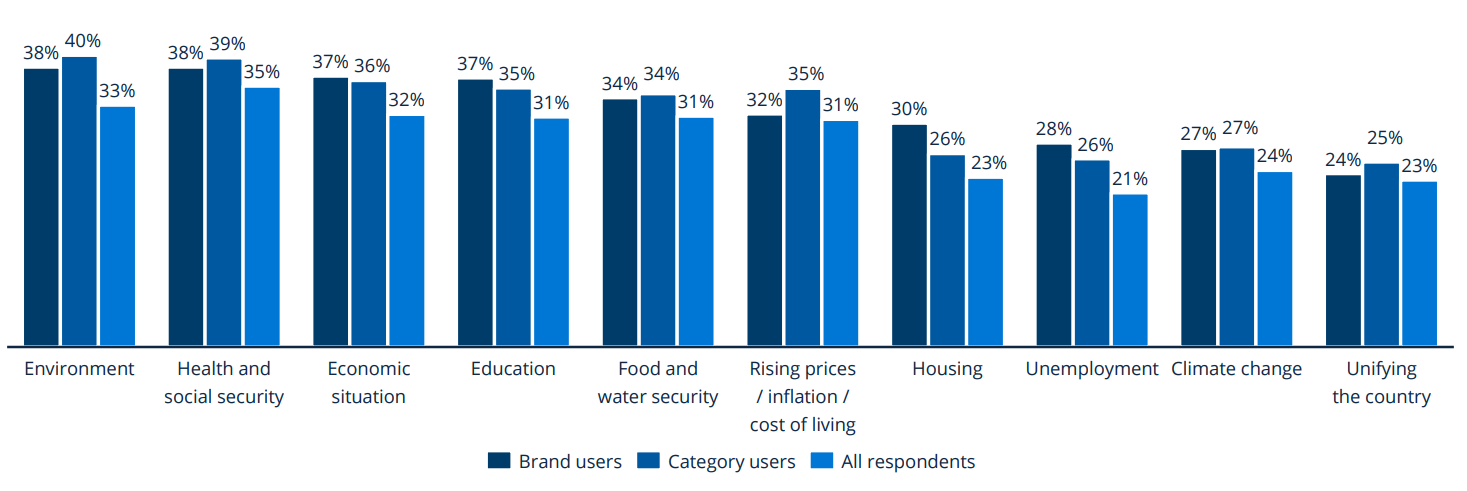
\includegraphics[width=1\textwidth]{Images/19.png}
    \caption{中国面临的十大重要问题(原问题:“What do you personally think are the most important issues in your country of residence that need to be addressed?”)\cite{34}}
    \label{china}
\end{figure}

环境是消费者们最关注的,“节俭意识”就自然萌芽了。近年,许多网站上都有关于购物节对环境的影响的报告,“反向消费”、“低碳生活”、“让绿色购物成为新时尚”、“可持续消费”...等等,这些说法并不少见。2018年,China Dialogue就发布的了以“Shopping festivals deliver disaster for environment”为题的一篇报告,以此来警示疯狂的消费者们;就在几天前,Make Fasion Better 发布了“Can Black Friday Go Green? The Environmental Cost of Excess Consumerism”的文章,很多媒体平台也经常表示对节俭的生活态度的支持,一来二去,更多的人也加入了这个队列。全球中产阶级不断增加、人口不断增长,能源需求增加和潜在成本增加让消费者感到了压力,超过60\%的人担心未来的生活成本会更高,因此选择向可持续的消费转变\cite{35}。



























\section{电商平台的应对措施}

为了适应消费者的行为变化,各大领头企业开始有针对性地设计一系列策略、各大品牌也接连出招。以可持续消费观念为例,在2022年,IKea将Black Friday转变为了“Green Friday”,鼓励消费者将不再需要的家具转卖给宜家,并赠予下次消费 50\% 折扣的优惠,这一举措得到了很好的响应,自 18 个月前建立该计划以来,IKea已向英国各地的人们提供了超过 51,000件重新利用的家具。另一个例子是户外服装销售商Patagonia,他们则在Black Friday提供额外的四项服务:保养与维修、二手物品购买、优质耐穿产品购买、社会回馈。Armani也将Black Friday打造成了“Blue Friday”,将其美妆网站上的每笔购买支出向“生命之水”计划\footnote{“生命之水”计划是2010年由Armani发起的,旨在为缺乏干净淡水的地区提供饮用水。}捐赠30\% \cite{22}。

\subsection{对比分析}
不妨将目光放到2021-2023这三年期间(也就是各大购物节销售额增长率大幅度下降的时间段),图(\ref{strategies}) 展示了各大电商平台对于消费者对购物节兴趣大减的问题的具体应对方案、开始时间,很容易可以发现,大部分电商平台的策略都围绕着以下两点:
\begin{itemize}
    \item \textbf{主观设置上 - 顺应消费者心理需求.} \\
    就像前面给的三个具体的例子一样,许多电商平台都接受了消费者向理性消费、绿色消费的转变,他们推出的策略则直接顺应了这两点,以情感共鸣改善消费者对购物节的负面观感。
    \item \textbf{客观设置上 - 分散购物或延长购物节时间.} \\
    也就是推行许多小型、分期促销活动,或者直接延长时间,给犹豫不决的消费者思考空间。
\end{itemize}

\begin{figure}[htbp!]
    \centering
    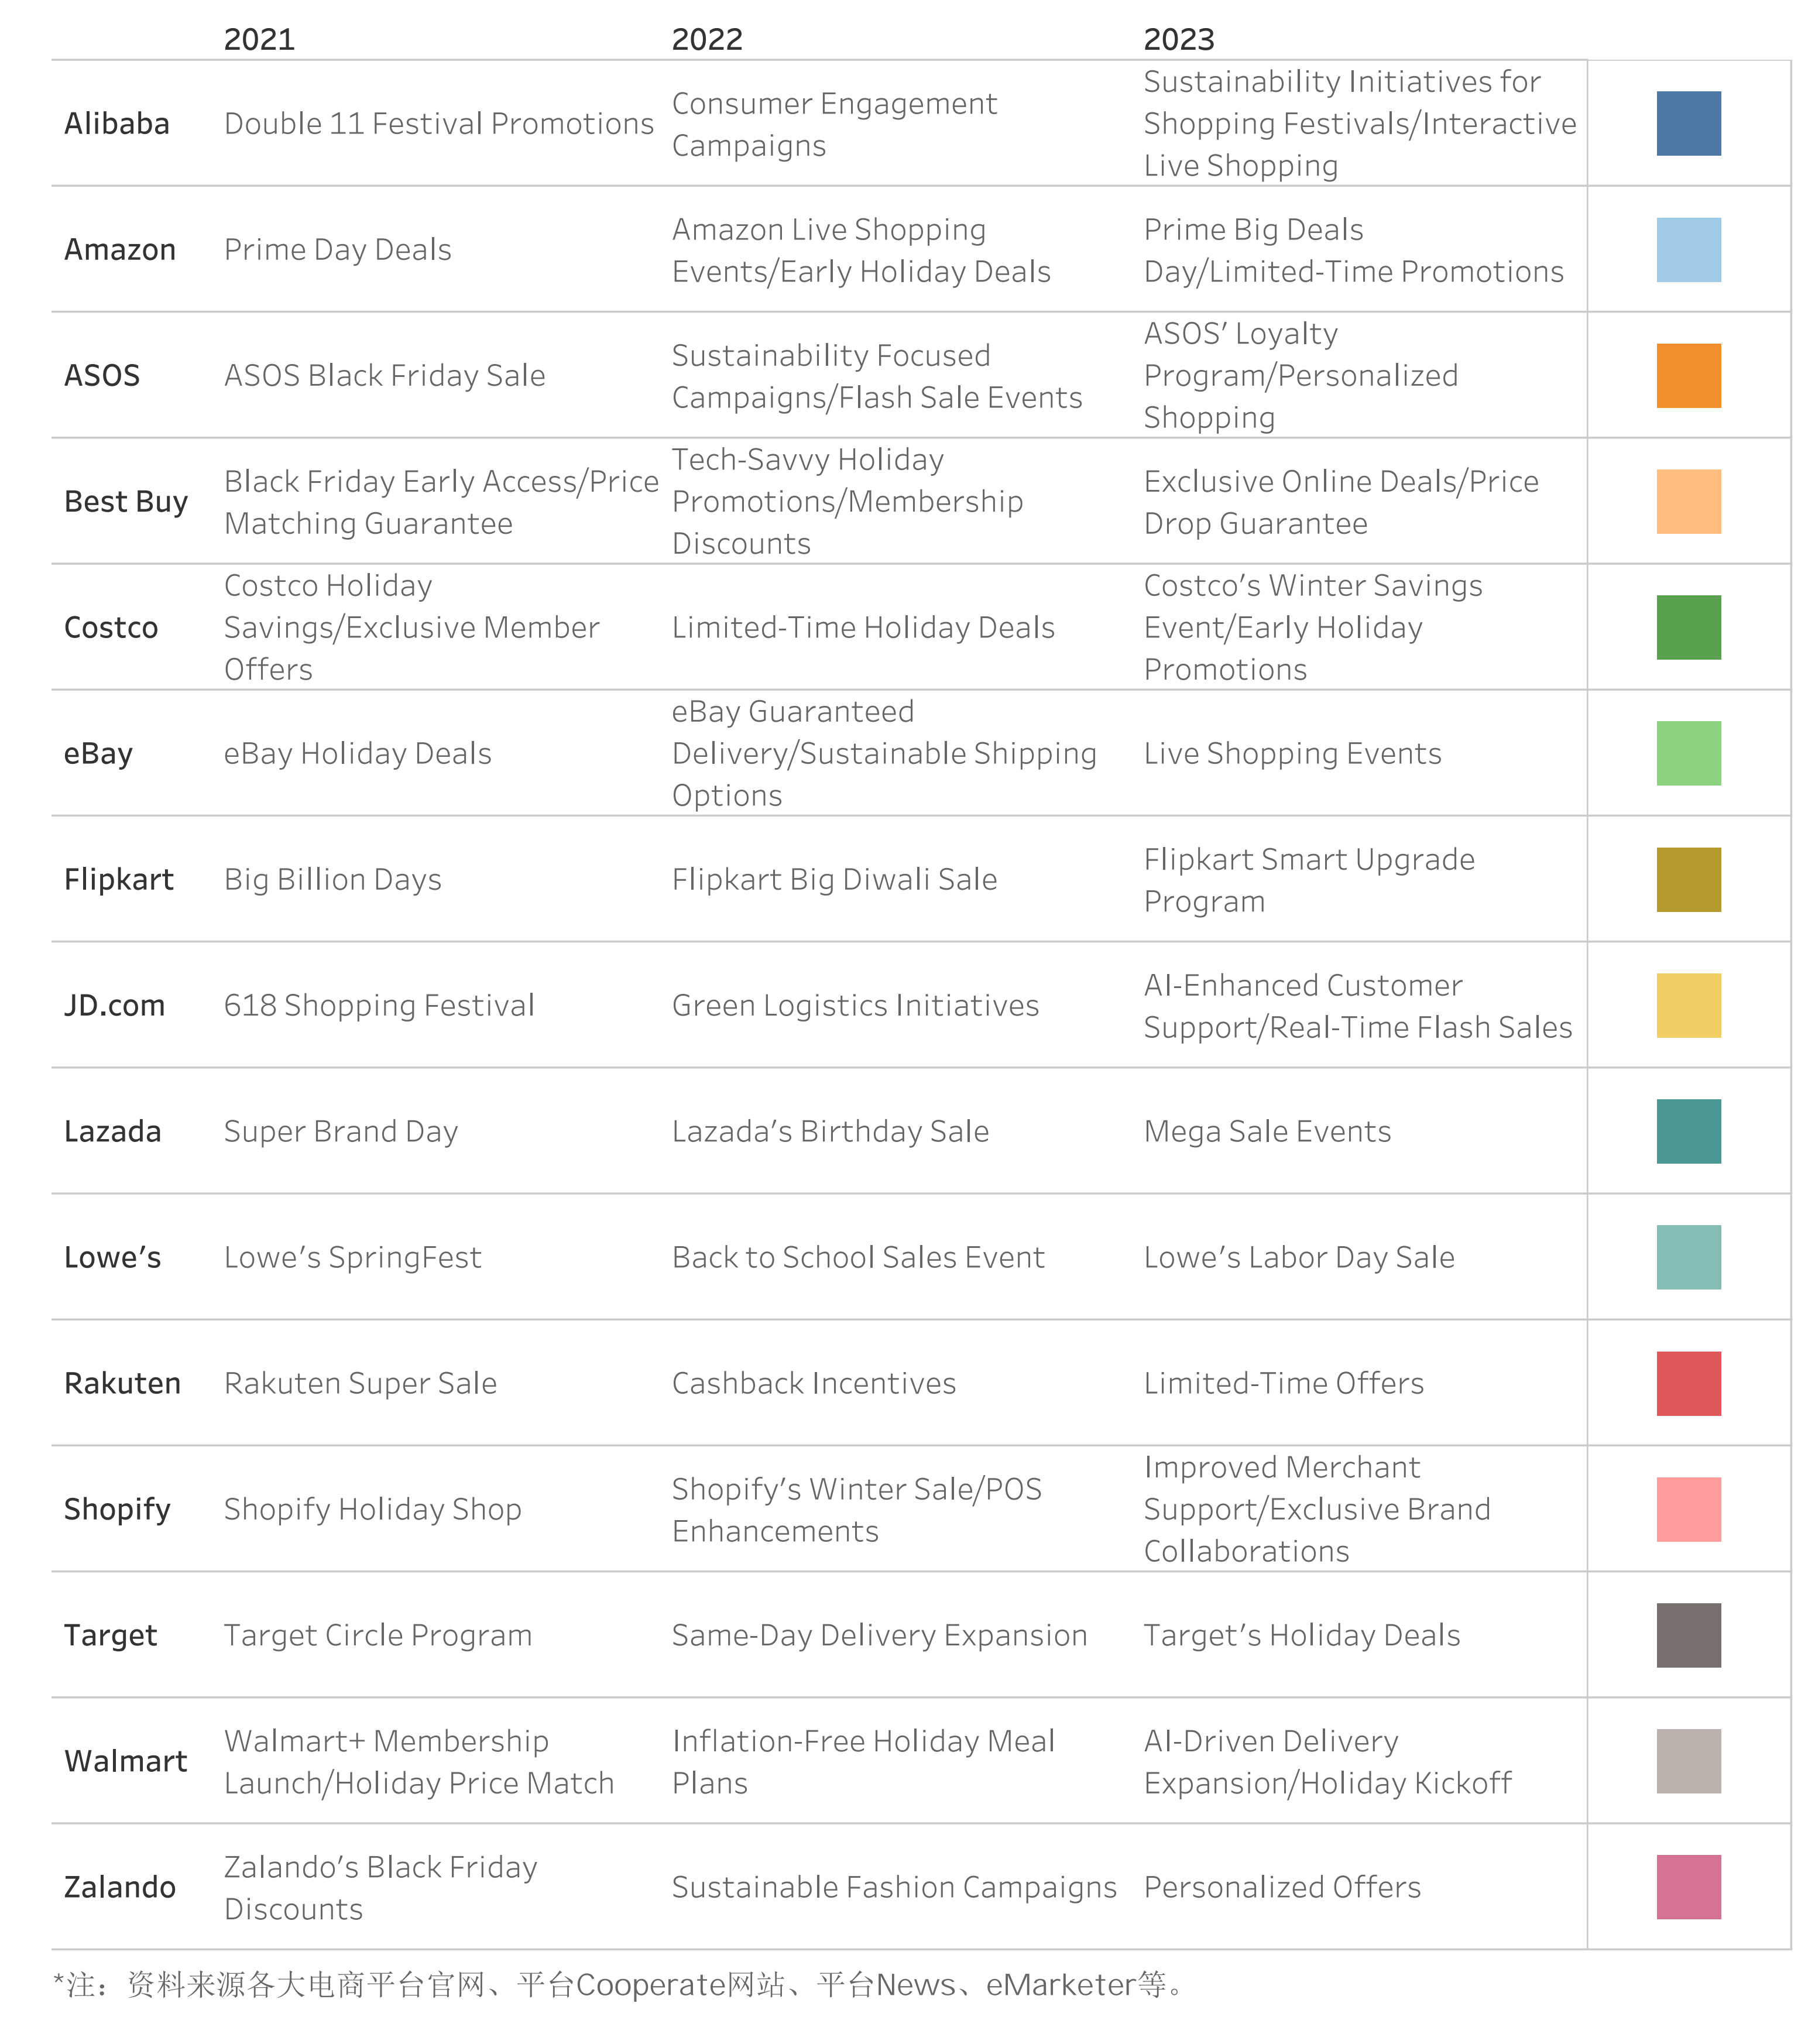
\includegraphics[width=1\textwidth]{Images/18.png}
    \caption{2021-2023年各主流电商平台就“消费者对购物节兴趣降低”问题的策略}
    \label{strategies}
\end{figure}

由图(\ref{strategies}),总的来看,Amazon、Best Buy、Costco、Flipkart、Lazada、Lowe's、Rakuten、Shopify、Targret、Walmart在近三年还未特地推出可持续性相关策略,更多的关注点还是放在了各种短长期购物节促销上;Alibaba、Amazon、eBay、JD.com都先后开始采用直播推广购物节的方式。这里给出的平台数量一共有十五个(按首字母顺序排列),为更清晰,下面单独将购物节的主流平台拎出来,结合实施效果对其策略进行横向、纵向对比分析。

\begin{itemize}
    \item \textbf{Alibaba vs Amazon.} \\
    Alibaba将精力更多花在提升用户体验上,以折扣结合社交互动型电商,从消费者视角满足需求,而Amazon则是开启多渠道推广,以直播、延长折扣活动、现时抢购等方式主动吸纳消费者。Amazon的Prime会员服务已经为其建立了良好的用户忠诚度,选择延展并且分散化促销的根本目的就是增多Prime会员注册数,以此反哺Prime Day(前文已提到数据)。
    \item \textbf{Amazon vs Best Buy.} \\
    Amazon 和 Best Buy 起初的策略是相似的,一个是延长折扣时间、另一个是提前开放折扣活动,本质上都是分散化促销。比较特别的是Best Buy在2022年推出的Tech-savvy Holiday Promotions,这个方案将目光聚焦于科技产品并提供捆绑销售,面向的是对电子设备、智能家居等感兴趣的消费者群体,这为占市场份额远不及Amazon的它带来了约10\%的增长率。
    \item \textbf{Best Buy vs eBay.} \\
    eBay走的策略路线则跟Best Buy相差较大,前者既回应了用户可持续心理又学习了直播促销模式,后者的策略则更为传统(如Price Drop Gaurantee是为了增强消费者信心)。Best Buy 其实也承诺使用环保包装材料,并尽可能减少运输过程中的碳排放,eBay则专门推行了Sustainable Shipping Options的策略,卖家可自行勾选碳中和运输选项,参与环保行动。
    \item \textbf{eBay vs JD.com.} \\
    eBay和JD.com在2022年似乎都察觉到了可持续性的需求,都推出了针对物流运输的环保类策略,但在2023年,两者不再相同。eBay的直播购物活动销售额比普通销售增长了20\%, JD.com的实时秒杀使销售额增长15\%,吸引了大量新用户注册;还以AI技术辅助服务。
    \item \textbf{JD.com vs Target.} \\
    Target的策略相较于JD.com就更偏向传统了,但是他们有一个共通的目的 - 提升品牌的社会责任形象,以提高消费者粘性来推动购物节。Target Circle Program允许消费者将积分用于支持社区或慈善机构;JD.com物流引入碳足迹追踪系统、推出可重复使用的“青流箱”。
    \item \textbf{Target vs Walmart.} \\
    Walmart和Target都在商品运输方面设计了策略,一个追求速度、另一个则追求智能化。2021年的Walmart+显然是效仿了Amazon的Prime服务,但它特别的的Inflation-free holiday meal plans就是对消费者的极大人文关怀了,直接针对低收入和中产阶级家庭的痛点,还能吸引价格敏感型消费者,食品销售额增长约10\%,Target的策略也就略显逊色了。
    \item \textbf{Walmart vs Alibaba.} \\
    Alibaba和Walmart这三年间的策略交际就比较少了(这是自然的,因为面向的市场不同,竞争强度更小),不过他们都就前面提到的主、客观设置在提升用户忠诚度上下了功夫。
\end{itemize}



\subsection{技术发展对策略布线的影响}

\begin{quote}
    \textit{“Invest like an attacker. You can't outsource your way to victory. Technology is strategy. You can't know your customers if you don't know AI. ”} \\
    \raggedleft \textit{- MicKensey \& Company \cite{42}}
\end{quote}

策略由消费者需求出发,而技术发展则是真正实策略的途径。不妨也从一些近期报道看起。

\subsubsection{人工智能与机器学习}
人工智能和大模型的出现可以说是为各大电商平台策略布线指引了一个无限可能的方向,因为它始终关乎“个性化购物体验”,从根本上来说,就是“客户至上”准则。

今年9月发布的一篇报告\cite{40}中说到,Walmart正在将新技术融入其电子商务计划,他们将添加一个生成式人工智能聊天机器人来管理客户服务(如“取消订单”、“启动退款”等),并在游戏平台 Roblox 上销售Walmart的商品,还会为每位用户提供个性化主页,将动态文本和动态图像整合在一起为客户创建定制的内容,这项技术已经在其美国网站和部分应用程序中开始使用。

同年9月的另一篇报告\cite{41}中也说,35\% 的公司正在使用人工智能为受众提供流畅的用户体验,51.9\% 的营销人员在 TikTok 上使用人工智能进行电子商务整合,预计到 2030 年,全球AI 电商市场将达到 168 亿美元,复合年增长率为 15.7\%。AI技术的发展将推进个性化策略的实施。

\begin{figure}[htbp!]
    \centering
    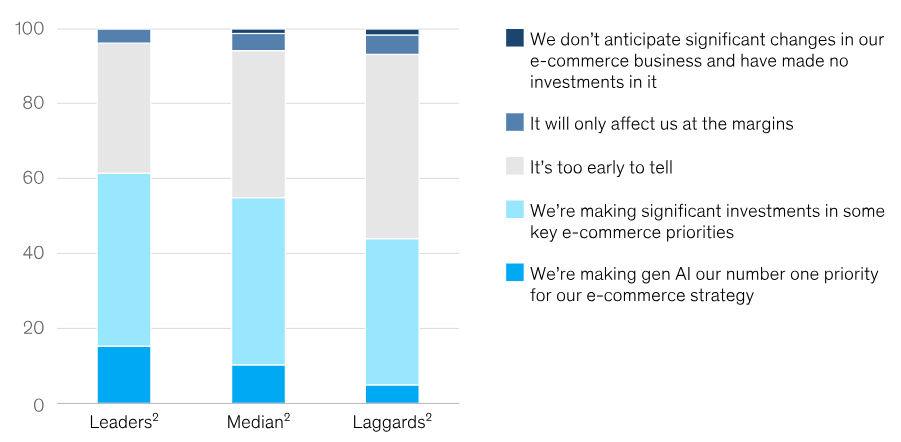
\includegraphics[width=0.8\textwidth]{Images/23.png}
    \caption{2024年MicKensy \& Company对各电商平台就生成式人工智能在电子商务中的角色观点的调研结果(原问题:“Which of the following statements best reflects your company's view of the role of generative AI in your business's e-commerce stratege?”)\cite{42}}
    \label{auto}
\end{figure}

由上图可以看出,超过60\%的电商领头公司都将AI的应用纳入前几重要的策略制定中。Amazon也将在今年10月整合 Anthropic 的Claude 模型来提高 Alexa 的响应效率和准确性\cite{44}。

在过去的2021-2023年也有很多例子(图(\ref{strategies}))。Amazon的Live Shopping Events使用的Interactive Video Service(IVS)服务集成了AI驱动和机器学习,对象检测、人脸识别、情绪识别是图像处理技术,而实时字幕、语音反馈则是自然语言处理技术;JD.com的AI-Enhanced Customer Support和Walmart的AI-Driven Delivery Expansion也是直接体现了AI对策略的导向作用。

\subsubsection{增强现实与虚拟现实技术}
增强现实(AR)与虚拟现实(VR)可以认为是人工智能的一个分支,但是上面提到的技术更侧重于基于数据的分析预测来迎合客户偏好,这里则更多涉及“更为直接”的客户体验。

\cite{40}中同样提到,Walmart推出了一项名为 Walmart Realm 的新体验,这是他们的首个沉浸式商业项目,他们还计划在拥有 2000 万活跃用户的社交平台 Zepeto 上推出虚拟品牌店,并提供 3D 头像定制。更普遍地来说,Shopify在今年8月发布的报告\cite{43}中预测, 2032 年AR/VR 市场将达到1.19 万亿美元,各大科技公司也在投资以加速这一趋势,如Google于 2022 年收购了研发智能眼镜的 Raxium、Apple收购了 AR 头戴设备初创公司 Mira,他们自己也推出了Shopify AR。



\subsubsection{区块链技术}
区块链技术为电商平台提供了更高的透明度,使消费者能够追踪产品的来源和运输过程,增强信任感,如IBM 就有 Food Trust 网络通过区块链技术追踪食品供应链来确保产品的安全和质量,它还可以被用于智能化合约自动化交易和简化支付流程。

今年,eBay就将一种突破性的用户身份验证方法引入区块链技术——“Blockchain-Based User Authentication: A Digital Handshake”,以此基于绩效奖励信誉并惩罚欺骗行为,以清除平台上损害其声誉的欺诈和假冒产品,提升自身平台口碑\cite{45}。还有Amazon的AWS(Amazon Web Services)、Alibaba的蚂蚁金服...,区块链技术的更新也在指引新策略的推出。















\subsection{今年行业动态侦测}
今年的购物节情况又会如何呢?不妨先看已经结束了的购物节,以及他们已经做了什么。

首先是最先结束的618购物节\footnote{在这之前还有春节促销、情人节促销、复活节促销、劳动节促销、母亲节促销等,但因为其与节假日更相关,就并不作为购物节来讨论了。},China Trading Desk的首席执行官表明热闹程度有所下降,但快时尚和高端时尚产品销量都有增长,环保产品以及个性化和定制时尚产品在这期间受到了消费者的青睐\cite{23}。阿里巴巴集团旗下的天猫(Tmall)采用的策略是忠诚度计划和高端商品的直接推出,以此吸引消费者。忠诚度计划的代表是88VIP,截至6月18日活动结束时,365个品牌的销售额已超过一亿人民币销售额,这得归功于65\%的88VIP新会员增长\cite{23}。天猫也在今年推出了 200 多个高端品牌,一改传统预售模式,直接向消费者提供独家产品,同时,还在消费激励上投入了至今最高的150亿人民币。京东(JD.com)的策略则是“大订单”计划,还邀请宝洁、SK-II、海尔等大公司的高管参与京东的直播,通过“红包雨”等福利吸引消费者,直播订单量增长超200\%。除了高管直播,还有数字人直播,京东云言犀数字人在超过 5,000 个品牌直播间带来了超过 1 亿的观看次数,9.9包邮频道也首次推出2元包邮日\cite{24},收益甚佳。6月17日晚,京东联合湖南卫视打造“京东618开心夜”晚会,期间,用户在京东的互动量超397亿\cite{24}。

第二是七月结束的Prime Day,eMarketer在今年五月发布的报告\cite{25}中提到,亚马逊在其日历中添加了几个小型促销活动,突出不同的类别和场合,以吸引消费者在Prime Day之前就开始消费,如3月20日至25日的春季大促销、5月7日至8日的宠物日、5月15日至5月20日的图书大促销、5月13日至5月19日的夏季美妆促销、5月20日至27日的阵亡将士纪念日促销。据 CivicScience 称,超过三分之一(36\%)的美国消费者参加了亚马逊今年的春季大促销,与 2023 年同期相比,销售额增长了 10.6\%,不仅如此,28\% 的非 Prime 会员春季大促销购物者在促销结束后注册成为了Prime会员!- 这无疑也是为Prime Day促销推广做准备。但就这次春季大促销来说,消费者行为似乎并不像主题所呼吁的“春季时装、健身产品以及清洁和庭院工作必需品”那样(只有10\%不到选择了它们),更多人还是在购买健康和美容、电子和技术以及家居、装饰品。不过总的来说今年的Prime Day收益甚佳,根据Forbes的报道,总销售额破纪录地达到了 142 亿美元,Fire TV 棒、Premier 蛋白奶昔和液体 IV 包是最受欢迎的商品,主要购物者是35-44 岁的高收入阶层居住在郊区的女性\cite{26}。

下面是今年还没举办的购物节,但是一些平台已经提前公布了他们的新策略。

第三是即将到来的"双十一”购物节,公布的策略大多围绕折扣力度、折扣方式,且折扣日期都较去年推前了近10天。10月9日,拼多多揭晓了他们的新“百亿消费券”策略,允许消费者在享受的百亿补贴价格基础上进一步叠加使用,最终支付价格最低可达原价的2.5折,“百亿加倍补”也将升级为“超级加倍补”\cite{27}。但不同于618,天猫将重启预售模式;淘宝在收到其618期间商家就“仅退款”的不满后将上线“退货宝”\cite{28}。也就是说,除了低价吸引用户,许多中国电商平台正在谋求商家和消费者的利益均衡。

第四个就是Black Friday和Cyber Monday(BFCM)了,Vogue Business在今年九月的预测认为消费者的信心会上升,这是一个好消息,但仍然需要激励谨慎的消费者花他们辛苦赚来的钱\cite{29}。他们还认为,中东的地缘政治冲突导致的部分亚欧苏伊士运河航线停运将影响折扣,昂贵的空运也会给零售利润带来压力。Walmart还是如往常一样,将在Black Friday提前给“Walmart+”客户开放折扣,不过,据Walmart官方透露,产品将新增高端美妆、收藏品、与StockX合作的运动鞋等,今年他们也将开启“Inflation-free Holiday Meal Weeks”,旨在缓解了消费者对高物价的担忧;他们还将引入新AI技术扩大其送货范围,预计涵盖额外的1200万户家庭,现在,他们已经公布了“2024年热门玩具清单”\cite{30}。亚马逊似乎还没有公布今年将新增的购物节推广措施,不过刚刚结束的从10月8日至9日的Prime Big Deal Day看来,早期销售策略一直走势良好。其他电商平台如Best Buy、Target等还未透露 2024 年BFCM的计划\cite{31}。

\subsection{购物节活动优化建议}

根据前文谈到的其他电商平台以应对消费者衰减的兴趣的购物节激励策略,结合\cite{26,32}的观点,本报告作者就亚马逊平台角度出发提出以下几个购物节活动优化拙见:

\begin{itemize}
    \item \textbf{赋予并提供真正的价值.} \\
    这里所说的“价值”不仅仅是商品本身的价值(或者说不仅是一直沿用的低价策略,当然低价策略非常重要,\cite{32}中提到Salsify调研的人群中36\% 将自己定义为“讨价还价猎人”),而是需要顺应大众对精简生活的追求、环保意识的逐渐萌发,给购物节本身赋予意义。就像Armani、Ikea做的那样,亚马逊也可以推出“可持续的Friday”,如 \textcolor{blue}{(I)} 在快递包装盒上做改进,使用可降解材料、简化包装、激励二次使用(如JD.com的“青流箱”)等;\textcolor{blue}{(II)} 配送服务使用电动或混合动力配送车,集中配送到指定站点,鼓励消费者前往配送站点自提(考虑到部分地区居民地分布松散,集中配送的方法或许并不适用)并奖励行为积分用于折扣或电子植树(如支付宝开展的公益活动);\textcolor{blue}{(III)} 专门设立绿色产品专区,标注商品的环保认证,以帮助犹豫不决的消费者做选择,且前调研显示他们也愿意支付溢价,平台则能获利平衡。
    \item \textbf{针对不同购物活动找到受众.} \\
    这里强调的是个性化推荐的作用,铺天盖地的“历史最低”、“闪电秒杀”等字眼会淹没消费者,不但催生厌烦情绪,转化率也会大大降低。可改进的方案如:\textcolor{blue}{(I)} 针对(广告设计风格也应符合该年龄段审美), A/B 测试优化推送策略;\textcolor{blue}{(II)} 采取不同推广方法,如对Z世代采用Tiktok宣传、Instagram广告播送,而对婴儿潮一代则加强零售店管理,给他们一个安全有序的购物节线下采购环境;\textcolor{blue}{(III)} 对特定人群推送特定商品信息,如对30-50岁的高收入阶层女性推送健康和美容类产品、对20-40岁的青壮年男性推送电子和技术类产品,也可以利用其收购的Twitch直播平台联动知名游戏主播(如:XQC、ImperialHal等)推广电子设备;\textcolor{blue}{(IV)} 引入LLM虚拟助手,通过聊天功能与用户实时互动,并且对服装、饰品类产品提供AR试穿、试戴功能,根据需求推送广告。
    \item \textbf{提供更多真实的产品信息.} \\
    这里的关键点在“真实”,以适应消费者的谨慎消费心理。不妨做以下改进:\textcolor{blue}{(I)} 除产品功能与规格,附上详细的使用说明、可能发生的问题、维护指南,不过分夸大优点也不能完全隐藏缺点,与其等待,不如直接为可能的问题提供明确的解决指导;\textcolor{blue}{(II)} 提供高分辨率的多角度图片及其演示视频,让消费者真正“看到”使用的效果(这里可以借鉴天猫、淘宝等平台的促销策略,与直播带货方式结合,邀请KOL测评、设置参与红包奖励等);\textcolor{blue}{(III)} 对重点的商品设立FAQ用户社区,保证社区不受卖家干扰但需要规定可评论买家的信用水平(如其行为积分、守信度等),在这里消费者们可以分享使用心得、建议和问题,构建一个有活力的产品社区,未来该产品的更新迭代也可在此发布问卷、综合使用者的反馈信息作为参考。
    \item \textbf{创造全渠道且更安全的体验.} \\
    这里的“全渠道”指的是线上线下购物节的连贯性,Salsify调研的人群中有接近一半(49\%)都喜欢这种“杂交”购物模式\cite{32}。对全渠道:\textcolor{blue}{(I)} 统一的线上线下购物平台,使消费者即使线下购物也能实时查询库存信息;\textcolor{blue}{(II)} 支持线下取货后自助线上付款,实时统计个人拿取货物种类与个数,添加至电子账单,省去排队结账拥挤(也就是“先取后付”)。对安全性:\textcolor{blue}{(I)} 增强身份验证,引入指纹或面部识别等生物识别技术,实时监控交易,当检测到高风险交易时,自动向消费者发送警报和确认请求;\textcolor{blue}{(II)} 提供虚拟信用卡、虚拟电话、虚拟邮箱选择服务,允许用户生成一次性支付卡号、手机号、邮箱地址等,数据加密,减少消费者受到网络诈骗的侵扰;\textcolor{blue}{(III)} 购物节期间推行类似于“退换宝”服务,支持无忧退换,同时加强配送人员进行背景调查。
\end{itemize}









































\newpage
\newgeometry{right=1in,left=1in,top=1in,bottom=0.75in}
\addcontentsline{toc}{section}{参考文献}
\begin{thebibliography}{99}

    \bibitem{1} Chi, J. (2021). \textit{[Double 11 sales]}. In \textit{Double 11 sales maintain momentum, as industry overhaul shows effect}. Global Times. \\ Retrieved October 8, 2024, from https://www.globaltimes.cn/page/202111/1238773.shtml
    
    \bibitem{2} Carnahan, D. (2020, October 13). \textit{Amazon Prime Day 2020 is estimated to bring in \$9.91 billion in worldwide sales}. Business Insider. \\ Retrieved October 8, 2024, from https://www.businessinsider.com/amazon-prime-day-will-generate-over-9-billion-in-sales-2020-10?r=US\&IR=T

    \bibitem{3} Sinuate Media. (2023, November 28). \textit{How consumer behavior changed in 2023}. \\ Retrieved October 7, 2024, from https://sinuatemedia.com/2023-consumer-behavior/ \\     \#:~:text=Individuals\%20are\%20making\%20more\%20deliberate,evolving\%20ethos\%20of \\ \%20conscientious\%20consumerism. 

    \bibitem{4} Richter, F. (2023, November 23). \textit{[Worldwide search interest for the terms "Black Friday" and "Cyber Monday" on Google Search]}. In \textit{Are people losing interest in Black Friday?} Statista. \\ Retrieved October 8, 2024, from https://www.statista.com/chart/16167/google-search\\-es-for-black-friday/

    \bibitem{5} Fokina, M. (2024, September 24).  \textit{Black Friday facts \& Cyber Monday stats [Report 2024]}. Tidio.  \\ Retrieved October 8, 2024, from https://www.tidio.com/blog/black-friday-trends/\#fact-9

    \bibitem{6} Gitlin, J. (n.d.). \textit{5 Black Friday statistics that explain why the big shopping day may not last}. SurveyMonkey Curiosity. \\ Retrieved October 9, 2024, from https://www.surveymonkey.com/curiosity/5-black-friday-statistics/

    \bibitem{7} Tighe, D. (2024, Feburary 22). How consumers feel about shopping on Black Friday in selected countries as of September 2018 [Graph]. In \textit{Statista}. \\ Retrieved October 8, 2024, from https://www.statista.com/statistics/956129/consumer-attitudes-selected-countries-participation-black-friday/

    \bibitem{8} Owen, V. (2023, November 1). \textit{True or false? Unmasking Gen Z's attitudes to Black Friday \& Cyber Monday}. Pion. \\ Retrieved October 8, 2024, from https://www.wearepion.com/blog-posts/true-or-false-unmasking-gen-zs-attitudes-to-black-friday-cyber-monday. (Last updated August 19, 2024)

    \bibitem{9} Wethrift. (2024, August 6). \textit{Black Friday \& Cyber Monday statistics \& trends 2024}. \\ Retrieved October 9, 2024, from https://www.wethrift.com/p/black-friday-cyber-monday-statistics/\#yearly-black-friday-cyber-monday-spend-revenue-history
    
    \bibitem{10} Thomas, L. (2021, November 30). \textit{Cyber Monday online sales drop 1.4\% from last year to \$10.7 billion, falling for the first time ever}. CNBC.  \\ Retrieved October 9, 2024, from https://www.cnbc.com/2021/11/30/cyber-monday-online-sales-drop-1point4percent-from-last-year-to-10point7-billion-falling-for-the-first-time-ever.html

    \bibitem{11} Webb, M. (2024, August 1). \textit{80+ Key Cyber Monday statistics you need to know to navigate deals and retail trends in 2024}. Techopedia. \\ Retrieved October 9, 2024, from https://www.techopedia.com/cyber-monday-statistics

    \bibitem{12} Drive Research. (2023). \textit{Cyber Week report [2023]}. Drive Research. \\ Retrieved October 9, 2024, from https://www.driveresearch.com/media/5843/drive-research-cyber-week-report-2023.pdf

    \bibitem{13} Stambor, Z. (2024, June 28). \textit{July is the new December as consumers expect big bargains during the dog days of summer}. eMarketer. \\ Retrieved October 9, 2024, from https://www.emarketer.com/content/retailers-launch-big-sales-july

    \bibitem{14} Aronson, G. (2023, July 27). \textit{Global consumers defy economic pressure: Amazon Prime Day 2023 sparks shopping frenzy}. NielsenIQ.  \\ Retrieved October 9, 2024, from https://nielseniq.com/global/en/insights/education/2023 \\ /amazon-prime-day-2023-recap/

    \bibitem{15} Yuen, M. (2024, July 26).  \textit{GWhat Amazon Prime Day 2024 says about consumer sentiment}. eMarketer.  \\ Retrieved October 9, 2024, from https://www.emarketer.com/content/what-amazon-prime-day-2024-says-about-consumer-sentiment

    \bibitem{16} Daxue Consulting. (2023, November 17). \textit{The changing dynamics of Double 11 in China}. Daxue Consulting.  \\ Retrieved October 9, from https://daxueconsulting.com/double-11-2023-in-china/

    \bibitem{17} Shanghai Observer. (2023, November 21). \textit{Has the ‘Double Eleven’ shopping festival lost its luster?} Sixth Tone.  \\ Retrieved October 9, from https://www.sixthtone.com/news/1014120

    \bibitem{18} ALTAVIA. (2021, December 17). \textit{Consumer fatigue: Is Double 11 still worth the effort?} LinkedIn. \\ Retrieved October 10, from https://www.linkedin.com/pulse/consumer-fatigue-double-11-still-worth-effort-altavia/

    \bibitem{19} 孔海丽, \& 白杨. (2023, November 11). \textit{“双十一”消费者行为调研报告:谁赢了综合性价比之战?} 21世纪经济报道. \\ Retrieved October 10, from https://www.21jingji.com/article/20231111/herald/d2fa233 \\ 7789f23b5da017e7245cfa426.html

    \bibitem{20} 德勤中国. (2023). \textit{2023中国消费者洞察与市场展望白皮书}. Deloitte. \\ Retrieved October 10, from https://www2.deloitte.com/content/dam/Deloitte/cn/Documents/\\consumer-business/deloitte-cn-cb-consumer-insight-zh-230118.pdf

    \bibitem{21} 杨大坤, Sanders, M., \& 唐克家. (2023).  \textit{2023年“双十一”:理性和感性双管齐下,赢得消费者青睐}. Bain \& Company.  \\ Retrieved October 10, from https://www.bain.cn/pdfs/202311081258074010.pdf

    \bibitem{22} PG Paper. (2022, November 25). \textit{Boycotting Black Friday: Are attitudes shifting towards sustainability?} PG Paper.  \\ Retrieved October 10, from https://www.pgpaper.com/boycotting-black-friday-are-attitudes-shifting-towards-sustainability/

    \bibitem{23} Zhang, J., \& Nan, L. (2024, June 22). \textit{618 festival insights: Brand lessons on Tmall and JD.com}. Jing Daily. \\ Retrieved October 10, from https://jingdaily.com/posts/618-festival-insights-tmall-and-jd-com

    \bibitem{24} 京东黑板报. (2024, June 19).  \textit{京东618超5亿用户下单 成交额、订单量齐创新高 京东直播订单量同比增长超200\%}. 微信. \\ Retrieved October 10, from https://mp.weixin.qq.com/s/8ZgnaTjDsMwKpoDr3fBatw

    \bibitem{25} Feger, A. (2024, May 21).  \textit{Amazon uses smaller sales events to keep consumers spending outside of Prime Day}. eMarketer.\\ Retrieved October 10, from  https://www.emarketer.com/content/amazon-uses-smaller-sales-events-keep-consumers-spending-outside-of-prime-day

    \bibitem{26} Incrementum Digital. (2024, August 2).  \textit{Amazon Prime Day 2024 recap: 7 marketing \& advertising tactics for brands}. LinkedIn. \\ Retrieved October 10, from https://www.linkedin.com/pulse/amazon-prime-day-2024-recap-7-marketing-advertising-xilve/

    \bibitem{27} 中国家电网. (2024, October 10). \textit{拼多多启动双十一大促 “百亿消费券”叠加“超级加倍补”}. 中国家电网. \\ Retrieved October 10, from 
    http://news.cheaa.com/2024/1010/641708.shtml

    \bibitem{28} 南方都市报. (2024, October 10). \textit{史上最早双十一来了!天猫重启预售,京东预热力度空前}. 南方都市报. \\ Retrieved October 10, from https://m.mp.oeeee.com/a/BAAFRD0000202410101007564.html

    \bibitem{29} Shoaib, M. (2024, September 30). \textit{Four predictions for Black Friday 2024}. Vogue Business. \\ Retrieved October 10, from https://www.voguebusiness.com/story/consumers/four-predictions-for-black-friday-2024

    \bibitem{30} Walmart Corporate. (2024, September 19). \textit{Walmart unveils its holiday plans with early shopping deals and affordable meals}. Walmart Corporate.  \\ Retrieved October 10, from https://corporate.walmart.com/news/2024/09/19/walmart-unveils-its-holiday-plans-with-early-shopping-deals-and-affordable-meals

    \bibitem{31} Magyar, D. (2024, October 6). \textit{When is Black Friday 2024? When to grab the best holiday deals from Walmart, Amazon, Best Buy, Target and more}. NJ.com. \\ Retrieved October 10, from https://www.nj.com/shopping-deals/2024/09/when-is \\ -black-friday-2024-when-to-grab-the-best-holiday-deals-from-walmart-amazon-best-buy-target-and-more.html\#:~:text=Target\%20Black\%20Friday\%20Sale,getting\%20\\ the\%20best\%20deal \%20around.
    
    \bibitem{32} Bonderud, D. (2024, July 25). \textit{Cyber Week, Cyber Monday, and Black Friday trends: How excited are shoppers this year?} Salsify. \\ Retrieved October 10, from https://www.salsify.com/blog/cyber-week-cyber-monday-and-black-friday-trends

    \bibitem{33} Barkho, G. (2023, December 4). \textit{'Black Friday' and 'Cyber Monday' have lost their meanings as brands extend promotions}. Modern Retail.  \\ Retrieved October 12, from https://www.modernretail.co/marketing/black-friday-and-cyber-monday-have-lost-their-meanings-as-brands-extend-promotions/

    \bibitem{34} Statista. (2024, September). \textit{E-book shops: Amazon customers in China [Graph]}. In \textit{Statista}. \\ Retrieved October 13, from https://www.statista.com/study/91175/e-book-shops-amazon-customers-in-china/

    \bibitem{35} Ericsson. (n.d.). \textit{10 hot consumer trends: Climate change impacting consumers}. Ericsson. \\ Retrieved October 13, from  https://www.ericsson.com/en/reports-and-papers/\\consumerlab/reports/10-hot-consumer-trends-climate-change-impacting-consumers

    \bibitem{36} Kearl, M. (2023, August 21). \textit{Top effects of inflation on consumer behavior: 2023 inflation trends}. Medallia. \\ Retrieved October 14, from https://www.medallia.com/blog/inflation-effects-consumer-behavior-data-trends/

    \bibitem{37} Williams, R. (2023, October 1).  \textit{Consumers are cautious about holiday shopping plans}. MediaPost.  \\ Retrieved October 14, from https://www.mediapost.com/publications/article/399901/\\consumers-are-cautious-about-holiday-shopping-plan.html?edition=135888

    \bibitem{38} Haller, K. (2020, November 17). \textit{What's in store for the 2020 US holiday shopping season?} IBM Newsroom. \\ Retrieved October 14, from https://newsroom.ibm.com/Whats-in-Store-for-the-2020-US-Holiday-Shopping-Season

    \bibitem{39} Boston Consulting Group. (2023, November 9). \textit{Record Black Friday predicted with 74\% of consumers planning to shop, as cost-of-living crisis drives hunt for bargains}. PR Newswire. \\ Retrieved October 14, from https://www.prnewswire.com/news-releases/record-black-friday-predicted-with-74-of-consumers-planning-to-shop-as-cost-of-living-crisis-drives-hunt-for-bargains-301982403.html

    \bibitem{40} Choudhary, V. (2024, October 9). \textit{Walmart is rewiring its e-commerce strategy with generative AI}. Retail Brew. \\ Retrieved October 14, from https://www.retailbrew.com/stories/2024/10/08/walmart-is-rewiring-its-e-commerce-strategy-with-generative-ai

    \bibitem{41} Mileva, G. (2024, September 2). \textit{How AI is reshaping the future of eCommerce in 2024}. Influencer Marketing Hub.  \\ Retrieved October 14, from https://influencermarketinghub.com/ai-ecommerce/

    \bibitem{42} Arora, A., Wang, K. W., Zemmel, R., \& Zimmermann, S. (2024, October 8). \textit{Power forward: Five make-or-break truths about next-gen e-commerce}. McKinsey \& Company. \\ Retrieved October 14, from https://www.mckinsey.com/capabilities/growth-marketing-and-sales/our-insights/power-forward-five-make-or-break-truths-about-next-gen-e-commerce

    \bibitem{43} Keenan, M. (2024, August 19). \textit{AR shopping: Top trends and apps for the future}. Shopify.  \\ Retrieved October 14, from https://www.shopify.com/enterprise/blog/augmented-reality-ecommerce-shopping

    \bibitem{44} Munene, K. (2024, September 3). \textit{Amazon to launch enhanced Alexa experience with Anthropic’s AI}. Crypto Times. \\ Retrieved October 14, from https://www.cryptotimes.io/2024/09/02/amazon-to-launch-enhanced-alexa-experience-with-anthropics-ai/

    \bibitem{45} Cromley, K. (2024, February 27). \textit{eBay’s Blockchain Leap: Revolutionizing Trust and Security in E-commerce}. CoinTrust. \\ Retrieved October 14, from https://www.cointrust.com/market-news/ebays-blockchain-leap-revolutionizing-trust-and-security-in-e-commerce
    
\end{thebibliography}


% \newpage
% \addcontentsline{toc}{section}{Appendix}
% \section*{Appendix} 
% This is Appendix. % 这里写附录



\end{document}
